\documentclass[oneside]{book}

\setcounter{tocdepth}{2}
\setcounter{secnumdepth}{3}

\usepackage[toc,page]{appendix}
\usepackage{minted}
\usepackage[english]{babel}
\usepackage{graphicx}
\usepackage{hyperref}
\usepackage{amsmath} % Required for some math elements 
\usepackage{pdflscape}
\usepackage{pdfpages}

\newminted[HaskellCode]{haskell}{fontsize=\footnotesize}

\begin{document}

\begin{titlepage}
	\centering
	
\includegraphics[width=0.60\textwidth]{./logo/UoN_Primary_Logo_RGB.png}\par\vspace{1cm}
	{\scshape\Large PhD Thesis\par}
	\vspace{1.5cm}
	%{\huge\bfseries Foundations Of Pure Functional \\ Agent-Based Simulation \par}
%	{\huge\bfseries Pure Functional Programming \\ In Agent-Based Simulation \par}
	{\huge\bfseries The Pure Functional Programming Paradigm \\ In Agent-Based Simulation \par}
	\vspace{2cm}
	{\Large Jonathan Thaler (4276122) \\ \itshape jonathan.thaler@nottingham.ac.uk \par}
	\vfill
	supervised by\par
	Dr. Peer-Olaf \textsc{Siebers} \\
	Dr. Thorsten \textsc{Altenkirch}

	\vfill

	{\large \today\par}
\end{titlepage}

\cleardoublepage

\section*{Abstract}
This thesis shows how to implement Agent-Based Simulations (ABS) using the \textit{pure} functional programming paradigm and what the benefits and drawbacks are when doing so. As language of choice, Haskell is used due to its modern nature, increasing use in real-world applications and \textit{pure} nature. The thesis presents various implementation techniques to ABS and then discusses concurrency and parallelism and verification and validation in ABS in a pure functional setting. Additionally the thesis briefly discusses the use of dependent types in ABS, to close the gap between specification and implementation - something the presented implementation techniques don't focus on.
Finally a case-study is presented which tries to bring together the insights of the previous chapters by replicating an agent-based model both in pure and dependently typed functional programming. The agent-based model which was selected was much discussed in ABS communities as it claimed to have solved a fundamental problem of economics but it was then found that the implementation had a number of bugs which shed doubt on the validity and correctness of the results. The thesis' case study investigates whether this failure could have happened in pure and dependent functional programming and is a further test to see of how much value functional programming is to ABS. 

%TODO: from the 2nd annual review i got the feedback that i need to come up with a more coherent thesis structure which tells a story: i need to make myself clear what story i want to tell with my phd and what research and publications i still need to do for that (identify chapters and to which extent they are already finished). Also I need to come up with a precise publication plan, focusing on writing papers early than doing research for a too long time and starting an early thesis writing. This is because any unpublished research is lost and every published research is a contribution to knowledge. "A good PhD is asking more questions than it answers."

\clearpage
\tableofcontents
\clearpage
\textit{To my parents for their unconditional love and support throughout all my life.}
\clearpage

\chapter*{Acknowledgements}
Peer-Olaf Siebers Supervisor
Thorsten Altenkirch Supervisor
FP Group, for always being open to discussions, keen to help.
Martin Handley and James Hey for working through my thesis and their feedback.
Ivan Perez for always having an open ear for questions, valuable discussions with him and his contributions.
Julie Greensmith for the valuable discussions and pointing me into right directions at important stages of the phd.

\section{Introduction}
There exists a large number of simulation packages which allow the convenient creation of System Dynamics simulations by straight-forward visual diagram creation. One simply creates stocks and flows, connects them, specifies the flow-rates and initial parameters and then runs the model. An example for such a visual diagram creation in the simulation package AnyLogic can be seen in Figure \ref{fig:sir_stockflow_diagram}.

\begin{figure}
	\centering
	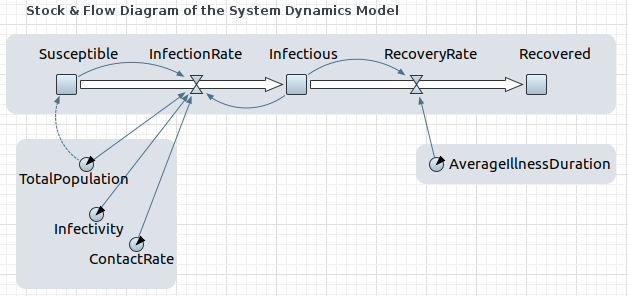
\includegraphics[width=.5\textwidth, angle=0]{./fig/SIR_SD_STOCKFLOW_DIAGRAMM.png}
	\caption{Visual System Dynamics Diagram of the SIR model in AnyLogic Personal Learning Edition 8.3.1.}
	\label{fig:sir_stockflow_diagram}
\end{figure}

Still, implementing System Dynamics directly in code is not as straight forward and involves numerical integration which can be quite tricky to get right. Thus, the aim of this paper is to look into how System Dynamics models can be implemented in code correctly without the use of a simulation package. We use the well known SIR model \cite{kermack_contribution_1927} from epidemiology to demonstrate our approach.

Our language of choice is Haskell because it emphasises a declarative programming style in which one describes \textit{what} instead of \textit{how} to compute. Further it allows to rule out interference with non-deterministic influences or side-effects already at compile-time. This is of fundamental importance for System Dynamics because it behaves completely deterministic and involves no stochastics or non-determinism whatsoever. Also, we make use of Functional Reactive Programming which allows to express continuous-time systems in a functional way. 

We show that by this approach we can arrive at correct-by-construction implementations of System Dynamic models. This means that the correctness of the code is obvious because we have closed the gap between the model specification and its implementation. Thus, the contribution of the paper is the demonstration of how to implement correct-by-construction System Dynamics simulations using Haskell and Functional Reactive Programming.

\section{Related research and literature}
\label{sec:literature}

The amount of research on using pure functional programming with Haskell in the field of ABS has been moderate so far. Most of the papers are related to the field of Multi Agent Systems (MAS) and look into how agents can be specified using the belief-desire-intention paradigm \cite{de_jong_suitability_2014,sulzmann_specifying_2007,jankovic_functional_2007}.

A multi-method simulation library in Haskell called \textit{Aivika 3} is described in the technical report \cite{sorokin_aivika_2015}. It supports implementing Discrete Event Simulations (DES), System Dynamics and comes with basic features for event-driven ABS which is realised using DES under the hood. Further it provides functionality for adding GPSS to models and supports parallel and distributed simulations. It runs within the IO effect type for realising parallel and distributed simulation but also discusses generalising their approach to avoid running in IO.

In his master thesis \cite{bezirgiannis_improving_2013} the author investigates Haskells' parallel and concurrency features to implement (amongst others) \textit{HLogo}, a Haskell clone of the NetLogo \cite{wilensky_introduction_2015} simulation package, focusing on using STM for a limited form of agent-interactions. \textit{HLogo} is basically a re-implementation of NetLogos API in Haskell where agents run within the IO context and thus can also make use of STM functionality. The benchmarks show that this approach does indeed result in a speed-up especially under larger agent-populations. The authors' thesis is one of the first on ABS using Haskell. Despite the concurrency and parallel aspect, this thesis approach is rather different: it avoids IO within the agents under all costs and explore the use of STM more on a conceptual level rather than implementing an ABS library to compare our case-studies with lock-based and imperative implementations.

There exists some research \cite{di_stefano_using_2005, varela_modelling_2004, sher_agent-based_2013} using the functional programming language Erlang \cite{armstrong_erlang_2010} to implement concurrent ABS. The language is inspired by the actor model \cite{agha_actors:_1986} and was created in 1986 by Joe Armstrong for Eriksson for developing distributed high reliability software in telecommunications. The actor model can be seen as quite influential to the development of the concept of agents in ABS, which borrowed it from Multi Agent Systems \cite{wooldridge_introduction_2009}. It emphasises message-passing concurrency with share-nothing semantics (no shared state between agents), which maps nicely to functional programming concepts. The mentioned papers investigate how the actor model can be used to close the conceptual gap between agent-specifications, which focus on message-passing and their implementation. Further they show that using this kind of concurrency allows to overcome some problems of low level concurrent programming as well.
Also \cite{bezirgiannis_improving_2013} ported NetLogos API to Erlang mapping agents to concurrently running processes, which interact with each other by message-passing. With some restrictions on the agent-interactions this model worked, which shows that using concurrent message-passing for parallel ABS is at least \textit{conceptually} feasible. Despite the natural mapping of ABS concepts to such an actor language, it leads to simulations, which despite same initial starting conditions, might result in different dynamics each time due to concurrency.

The work \cite{lysenko_framework_2008} discusses a framework, which allows to map Agent-Based Simulations to Graphics Processing Units (GPU). Amongst others they use the SugarScape model \cite{epstein_growing_1996} and scale it up to millions of agents on very large environment grids. They reported an impressive speed-up of a factor of 9,000. Although their work is conceptually very different this thesis draws inspiration from their work in terms of performance measurement and comparison to the Sugarscape model.

% THIS IS MY OWN REASEARCH, DON'T CITE IT HERE
%In \cite{thaler_pure_2019} the authors showed how to implement a spatial SIR model in pure Haskell using Functional Reactive Programming \cite{hudak_arrows_2003}. They report quite low performance but mention that STM may be a way to considerably speed up the simulation. We follow their approach in implementation technique, using Functional Reactive Programming and Monadic Stream Functions \cite{perez_functional_2016} (we don't go into implementation details as it is out of the scope of this paper) and use the spatial SIR model as the first case-study.

Using functional programming for DES was discussed in \cite{jankovic_functional_2007} where the authors explicitly mention the paradigm of Functional Reactive Programming (FRP) to be very suitable to DES.

A domain-specific language for developing functional reactive agent-based simulations was presented in \cite{schneider_towards_2012,vendrov_frabjous_2014}. This language called FRABJOUS is human readable and easily understandable by domain-experts. It is not directly implemented in FRP/Haskell but is compiled to Haskell code which they claim is also readable. This supports that FRP is a suitable approach to implement ABS in Haskell. Unfortunately, the authors do not discuss their mapping of ABS to FRP on a technical level, which would be of most interest to functional programmers.

Object-oriented programming and simulation have a long history together as the former one emereged out of Simula 67 \cite{dahl_birth_2002}, which was created for simulation purposes. Simula 67 already supported DES and was highly influential for today's object-oriented languages. Although the language was important and influential, in our research we look into different approaches, orthogonal to the existing object-oriented concepts.

Lustre is a formally defined, declarative and synchronous dataflow programming language for programming reactive systems \cite{halbwachs_synchronous_1991}. While it has solved some issues related to implementing ABS in Haskell, it still lacks a few important features necessary for ABS. There seems to be no way of implementing an environment in Lustre as it is done in Chapters \ref{ch:timedriven} and \ref{ch:eventdriven}. Also, the language seems not to come with stochastic functions, which are but the very building blocks of ABS. Finally, Lustre does only support static networks, which is clearly a drawback in ABS in general where agents can be created and terminated dynamically during simulation.

In \cite{botta_time_2010}, the authors discuss the problem of advancing time in message-driven agent-based socio-economic models. They formulate purely functional definitions for agents and their interactions through messages. Our architecture for synchronous agent-interaction as discussed in Chapter \ref{sec:eventdriven_implementation} was not directly inspired by their work but has some similarities: the use of messages and the problem of when to advance time in models which allows unrestricted synchronised agent interactions.

The authors of \cite{botta_functional_2011} are using functional programming as a specification for an agent-based model of exchange markets but leave the implementation for further research where they claim that it requires dependent types. This paper is the closest usage of dependent types in agent-based simulation we could find in the existing literature and to our best knowledge there exists no work on general concepts of implementing pure functional agent-based simulations with dependent types. %As a remedy to having no related work to build on, we looked into works which apply dependent types to solve real world problems from which we then can draw inspiration from.

In his talk \cite{sweeney_next_2006}, Tim Sweeney CTO of Epic Games discussed programming languages in the development of game engines and scripting of game logic. Although the fields of games and ABS seem to be very different, Gregory \cite{gregory_game_2018} defines computer-games as \textit{"[..] soft real-time interactive agent-based computer simulations"} (p. 9) and indeed, they have striking similarities: both are simulations which perform numerical computations and update objects in a loop either concurrently or sequential. In games these objects are called \textit{game-objects} and in ABS they are called \textit{agents} but they are conceptually the same thing.  Sweeney reports that reliability suffers from dynamic failure in languages like C++ e.g. random memory overwrites, memory leaks, accessing arrays out-of-bounds, dereferencing null pointers, integer overflow, accessing uninitialized variables. He reports that 50\% of all bugs in the Game Engine Middleware Unreal can be traced back to such problems and presents dependent types as a potential rescue to those problems. The two main points Sweeney made were that dependent types could solve most of the run-time failures and that parallelism is the future for performance improvement in games. He distinguishes between pure functional algorithms which can be parallelised easily in a pure functional language and updating game-objects concurrently using Software Transactional Memory (STM).

\chapter{Methodology}
This chapter introduces the background and methodology used in the following chapters. Roughly 50\% exists already.

\section{Agent-Based Simulation}
History, methodology (what is the purpose of ABS: 3rd way of doing science: exploratory, helps understand real-world phenomena), classification according to \cite{macal_everything_2016}, ABS vs. MAS, event- vs. time-driven \cite{meyer_event-driven_2014}, examples: agent-based SIR, SugarScape, Gintis Bartering

\subsection{Traditional approaches}
Introduce established implementation approaches to ABS. Frameworks: NetLogo, Anylogic, Libraries: RePast, DesmoJ. Programming: Java, Python, C++. Correctness: ad-hoc, manual testing, test-driven development.

\subsection{Verification \& Validation}
Introduction Verification \& Validation (V \& V in the context of ABS).

%--------------------------------------------------------------------------

\section{Pure functional programming}
Definition, Haskell references,

In our research we are using the \textit{pure} functional programming language Haskell. The paper of \cite{hudak_history_2007} gives a comprehensive overview over the history of the language, how it developed and its features and is very interesting to read and get accustomed to the background of the language. The main points why we decided to go for Haskell are:

\begin{itemize}
	\item Rich Feature-Set - it has all fundamental concepts of the pure functional programming paradigm included. Further, Haskell has influenced a large number of languages, underlining its importance and influence in programming language design.
	\item Real-World applications - the strength of Haskell has been proven through a vast amount of highly diverse real-world applications \cite{hudak_haskell_1994, hudak_history_2007}, is applicable to a number of real-world problems \cite{osullivan_real_2008} and has a large number of libraries available \footnote{\url{https://wiki.haskell.org/Applications_and_libraries}}.
	\item Modern - Haskell is constantly evolving through its community and adapting to keep up with the fast changing field of computer science. Further, the community is the main source of high-quality libraries.
	\item Purity - Haskell is a \textit{pure} functional language and in our research it is absolutely paramount, that we focus on \textit{pure} functional ABS, which avoids any IO type under all circumstances (exceptions are when doing concurrency but there we restrict most of the concepts to STM).
	\item It is as closest to pure functional programming, as in the lambda-calculus, as we want to get. Other languages are often a mix of paradigms and soften some criteria / are not strictly functional and have different purposes. Also Haskell is very strong rooted in Academia and lots of knowledge is available, especially at Nottingham, 
		Lisp / Scheme was considered because it was the very first functional programming language but deemed to be not modern enough with lack of sufficient libraries. Also it would have given the 
		Erlang was considered in prototyping and allows to map the messaging concept of ABS nicely to a concurrent language but was ultimately rejected due to its main focus on concurrency and not being purely functional.
		Scala was considered as well and has been used in the research on the Art Of Iterating paper but is not purely functional and can be also impure.
\end{itemize}


\subsection{Functional Reactive Programming}
Short introduction to FRP (yampa), based on my pure functional epidemics paper.

\subsection{Monadic Stream Functions}
Short introduction to MSFs (dunai), based on my pure functional epidemics paper.

\section{Dependent Types}
Example, Equality as Type, Philosophical Foundations: Constructive mathematics

\section{Implementing ABS}
\label{ch:impl_abs}
In this section we briefly present a general background on problems and considerations, ABS implementations need to solve independent from the programming paradigm. In general, an ABS implementation must solve the following fundamental problems:

\begin{enumerate}
	\item How to represent an agent, its local state and its interface.
	\item How to represent agent-to-agent interactions and enforcing their semantics.
	\item How to represent an environment.
	\item How to represent agent-to-environment interactions and enforcing their semantics.
	\item How agents and an environment can initiate actions without external stimuli.
	\item How to step the simulation.
\end{enumerate}

% agent- and environment pro-activity
We argue that the most fundamental concept of ABS is the \textit{pro-activity} of both, agents and its environment. In computer systems, pro-activity, the ability to initiate actions on its own without external stimuli, is only possible when there is some internal stimulus, most naturally represented by a continuous increasing time-flow. Due to the discrete nature of computer systems, this time-flow must be discretized in steps as well and each step must be made available to the agent, acting as the internal stimulus. This allows the agent then to perceive time and become proactive depending on time. So we can understand an ABS as a discrete time simulation where time is broken down into continuous, real-valued or discrete natural-valued time steps. Independent of the representation of the time-flow we have the two fundamental choices whether the time-flow is local to the agent or whether it is a system-global time-flow. Time-flows in computer systems can only be created through threads of execution where there are two ways of feeding time-flow into an agent. Either it has its own thread-of-execution or the system creates the illusion of its own thread-of-execution by sharing the global thread sequentially among the agents where an agent has to yield the execution back after it has executed its step. %Note the similarity to an operating system with cooperative multitasking in the latter case and real multiprocessing in the former.

% time- and event-driven ABS
Generally, there exist time- and event-driven approaches to ABS \cite{meyer_event-driven_2014}. In time-driven ABS, time is explicitly modelled and is the main driver of the ABS dynamics. The semantics of models using this approach, center around time. As a representative example, which will be used in Chapter \ref{ch:timedriven}, we use the agent-based SIR model \cite{macal_agent-based_2010, thaler_pure_2018}. Often such models are inspired by an underlying System Dynamics approach, where the continuous time-flow is the main driving force of the dynamics. It is clear that almost every ABS models time in some way, after all, modelling a virtual system over some (virtual) time is the very heart of Simulation. Still we want to distinguish clearly between different semantics of time representation in ABS: when time is seen as a continuous flow such as in the example of the agent-based SIR model, we talk about a truly time-driven approach. In other words: if an agent behaves as a time signal then we speak of a time-driven approach. This means that if the system is sampled with a $\Delta t = 0$ then, even though the agents are executed their behaviour must stay constant and must not change.

In the case where time advances in a discrete way either by means of events or messages, we talk about an event-driven approach. As a representative example, which will be used in Chapter \ref{ch:eventdriven} on event-driven ABS, we use an event-driven SIR and the Sugarscape model. In this model time is discrete and represented by the natural numbers where agents act in every tick. In such a model, the underlying semantics map more naturally to a Discrete Event Simulation core, extended by ABS features, as in the event-driven SIR and to a lesser extent in the Sugarscape model.

% agent representation
According to the definition of ABS in  Chapter \ref{sec:method_abs}, an agent is a uniquely addressable entity with an identity, an internal state it has exclusive control over and can be interacted with by means of messages. In the established object-oriented approaches to ABS all this is implemented naturally by the use of objects: an object has a clear identity, encapsulates internal state and exposes an interface through public methods through which objects can interact with each other, also called messaging. The same applies to the environment and it is by no means clear how to achieve this in a pure functional approach where we don't have objects available. This is one of the central questions this thesis is trying to answer and it will be addressed in the subsequent Chapters \ref{ch:timedriven} and \ref{ch:eventdriven}.

Before we look into pure functional ABS implementation concepts in the next chapters, we need to discuss the concept of update strategies \cite{thaler_art_2017}. Generally, there are four strategies to approach time- and event-driven ABS, where the differences deal with how the simulation is stepped, the agents are executed and the interaction semantics work.

% agent-to-agent interaction ant its semantics
%The semantics of messaging define when sent messages are visible to the receivers and when the receivers process them. Message-processing could happen either immediately or delayed, depending on how message-delivery works. There are two ways of message-delivery: immediate or queued. In the case of immediate message-deliver the message is sent directly to the agent without any queuing in between e.g. a direct method-call. This would allow an agent to immediately react to this message as this call of the method transfers the thread-of-execution to the agent. This is not the case in the queued message-delivery where messages are posted to the message-box of an agent and the agent proactively processes the message-box at regular points in time. With established OOP approaches we can have both: either a direct method-call or a message-box approach - in pure functional programming this is a much more subtle problem and it turns out that the problem of messaging / interacting of agents and of agents with the environment is the most subtle problem when approaching ABS from a pure functional perspective.

\subsection{Sequential strategy}
\label{sec:seq_strategy}
In this strategy there exists a globally synchronized time-flow and in each time step the simulation iterates through all the agents and updates one agent after another. Messages sent and changes to the environment made by agents are visible immediately, meaning that if an agent sends messages to other agents or changes the environment, agents which are executed after this agent will see these changes within the same time step. There is no source of randomness and non-determinism, rendering this strategy to be completely deterministic in each step. Messages can be processed either immediately or queued depending on the semantics of the model. If the model requires to process the messages immediately the model must be free of potential infinite-loops. Often in such models, the agents are shuffled when the model semantics require to average out the advantage of being executed as first. This strategy is of fundamental importance for event-driven ABS in Chapter \ref{ch:eventdriven}. See Figure \ref{fig:strategy_seq} for a visualisation of the control flow in this strategy.

\begin{figure}[H]
	\centering
	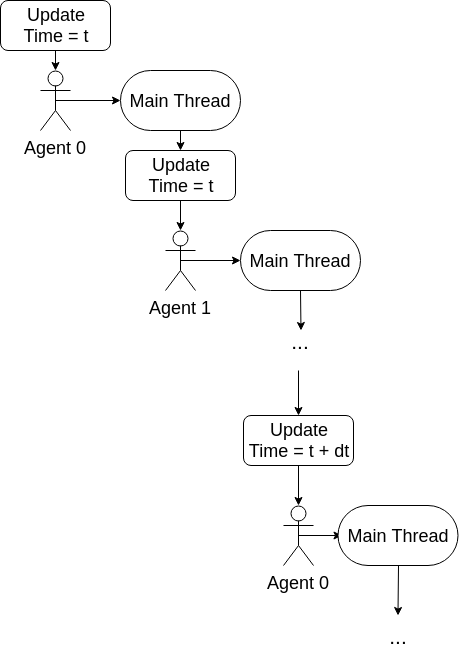
\includegraphics[width=0.5\textwidth, angle=0]{./fig/implabs/sequential.png}
	\caption[Control flow in the sequential update strategy]{Control flow in the sequential update strategy.}
	\label{fig:strategy_seq}
\end{figure}

\subsection{Parallel strategy}
\label{sub:par_strategy}
This strategy has a globally synchronized time-flow and in each time step iterates through all the agents and updates them in parallel. Messages sent and changes to the environment made by agents are visible in the next global step. We can think about this strategy in a way that all agents make their moves at the same time.  If one wants to change the environment in a way that it would be visible to other agents this is regarded as a semantic error in this strategy. First, it is not logical because all actions are meant to happen at the same time and second, it would implicitly induce an ordering, violating the semantics of the model, the \textit{happens at the same time} idea.
It does not make a difference if the agents are really executed in parallel or just sequentially - due to the isolation of information, this has the same effect. Also it will make no difference if we iterate over the agents sequentially or randomly, the outcome has to be the same: the strategy is event-ordering invariant as all events and updates happen \textit{virtually at the same time}. This strategy is of fundamental importance for time-driven ABS in Chapter \ref{ch:timedriven}. See Figure \ref{fig:strategy_par} for a visualisation of the control flow in this strategy.

\begin{figure}[H]
	\centering
	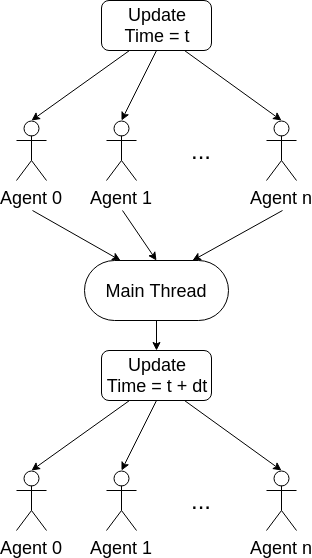
\includegraphics[width=0.4\textwidth, angle=0]{./fig/implabs/parallel.png}
	\caption[Control flow in the parallel update strategy]{Control flow in the parallel update strategy.}
	\label{fig:strategy_par}
\end{figure}

\subsection{Concurrent strategy}
\label{sub:con_strategy}
This strategy has a globally synchronized time-flow but in each time step all the agents are updated in parallel with messages sent and changes to the environment are visible immediately. So this strategy can be understood as a more general form of the \textit{parallel strategy}: all agents run at the same time but act concurrently. It is important to realize that when running agents, which are able to see actions by others immediately, in parallel, we arrive at the very definition of concurrency: parallel execution with mutual read and write access to shared data. Of course this shared data access needs to be synchronized which in turn will introduce event orderings in the execution of the agents. At this point we have a source of inherent non-determinism: although when one ignores any hardware model of concurrency, at some point we need arbitration to decide which agent gets access to a shared resource first, arriving at non-deterministic solutions. This has the very important consequence that repeated runs with the same configuration of the agents and the model may lead to different results. This strategy is of fundamental importance for concurrent ABS in Chapter \ref{ch:concurrent_abs}. See Figure \ref{fig:strategy_conc} for a visualisation of the control flow in this strategy.

\begin{figure}[H]
	\centering
	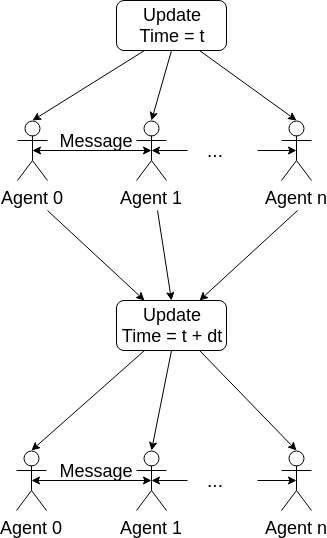
\includegraphics[width=0.5\textwidth, angle=0]{./fig/implabs/concurrent.png}
	\caption[Control flow in the concurrent update strategy]{Control flow in the concurrent update strategy.}
	\label{fig:strategy_conc}
\end{figure}

\subsection{Actor strategy}
\label{sub:act_strategy}
This strategy has no globally synchronized time-flow but all the agents run concurrently in parallel, with their own local time-flow. The messages and changes to the environment are visible as soon as the data arrive at the local agents - this can be immediately when running locally on a multiprocessor or with a significant delay when running in a cluster over a network. Obviously this is also a non-deterministic strategy and repeated runs with the same agent and model configuration may (and will) lead to different results. Information and also time in this strategy is always local to an agent as each agent progresses in its own speed through the simulation. In this case one needs to explicitly \textit{observe} an agent when one wants to extract information from it, for example for visualisation purposes. This observation is then only valid for this current point in time, local to the observer but not to the agent itself, which may have changed immediately after the observation. This implies that we need to sample our agents with observations when wanting to visualize them, which would inherently lead to well known sampling issues. A solution would be to invert the problem and create an observer agent which is known to all agents where each agent sends a \textit{'I have changed'} message with the necessary information to the observer if it has changed its internal state. This also does not guarantee that the observations will really reflect the actual state the agent is in but is a remedy against the notorious sampling. The concept of Actors was proposed by \cite{hewitt_universal_1973} for which \cite{grief_semantics_1975} and \cite{clinger_foundations_1981} developed semantics of different kinds. These works were very influential in the development of the concepts of agents and and can be regarded as foundational basics for ABS. We come back to this strategy in the context of concurrent ABS in Chapter \ref{ch:concurrent_abs}. See Figure \ref{fig:strategy_act} for a visualisation of the control flow in this strategy.

\begin{figure}[H]
	\centering
	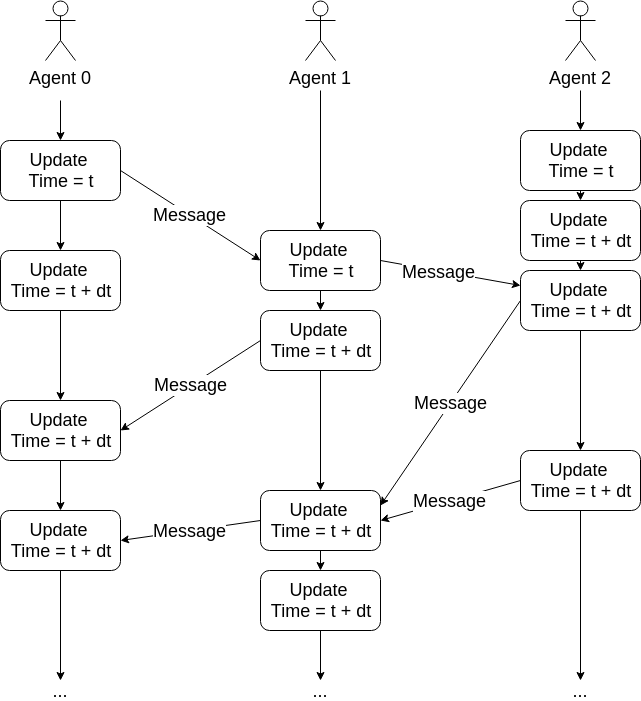
\includegraphics[width=0.5\textwidth, angle=0]{./fig/implabs/actor.png}
	\caption[Control flow in the actor update strategy]{Control flow in the actor update strategy.}
	\label{fig:strategy_act}
\end{figure}

\subsection{Discussion}
In the following chapters we discuss \textit{how} to implement ABS from a pure functional perspective and \textit{why} one would do so. More specifically, we show how to approach the problems discussed in this chapter using pure functional programming. The \textit{sequential} strategy will be covered in depth in Chapter \ref{ch:eventdriven} on event-driven ABS, the \textit{parallel} one in Chapter \ref{ch:timedriven} on time-driven ABS and the \textit{concurrent} strategy is used in Chapter \ref{ch:concurrent_abs} on concurrent ABS. The \textit{actor} strategy is not used in this thesis but its implementation follows directly from the Chapters \ref{ch:timedriven} and \ref{ch:concurrent_abs}: instead of globally synchronising in the main thread, a closed feedback loop is run in every agent thread. 

As already outlined in Chapter \ref{sec:method_abs}, the established approaches implementing ABS use object-oriented programming and thus solve the problems outlined at the start of this chapter from this perspective, which is quite well understood by now, as high quality ABS frameworks like RePast \cite{north_complex_2013} prove. In object-oriented programming an agent is mapped directly onto an object, encapsulating the agents state and providing methods, which implement the agents' actions. Object-orientation allows to expose a well-defined interface using public methods by which one can interact with the agent and query information from it. Agent objects can directly invoke other agents' methods, implicitly mutating the other agents' internal state, which makes direct agent interaction straight forward. Also with object-orientation, agents have global access to an environment for example through a Singleton \cite{gamma_design_1994} or a simple global variable, and can mutate the environments data by direct method calls.

All these language features are not available in functional programming and compared to object-orientation we face seemingly severe restrictions like immutable state, recursion and a static type system. Further, we restrict ourselves deliberately to \textit{pure} functional programming and avoid running in the non-deterministic \texttt{IO} Monad under all costs. The question is then how to solve these problems in functional programming \textit{and} use the restrictions to our advantage. In the next two chapters we show how to implement both a time-driven ABS  using the agent-based SIR model as example (Chapter \ref{ch:timedriven}) and an event-driven ABS using also the SIR and the complex Sugarscape model as examples (Chapter \ref{ch:eventdriven}). In both we present fundamental concepts of how to engineer an ABS from a pure functional programming perspective. This will then be used in subsequent chapters to discuss \textit{why} one would follow a  functional programming approach, identifying its benefits, advantages and also drawbacks over object-oriented approaches. 

%An implementation of an ABS must solve two fundamental problems:
%
%\begin{enumerate}
%	\item \textbf{Source of pro-activity} How can an agent initiate actions without the external stimuli of messages?
%	\item \textbf{Semantics of Messaging} When is a message \textit{m}, sent by agent \textit{A} to agent \textit{B}, visible and processed by \textit{B}?
%\end{enumerate}
%
%In computer systems, pro-activity, the ability to initiate actions on its own without external stimuli, is only possible when there is some internal stimulus, most naturally represented by a continuous increasing time-flow. Due to the discrete nature of computer-system, this time-flow must be discretized in steps as well and each step must be made available to the agent, acting as the internal stimulus. This allows the agent then to perceive time and become proactive depending on time. So we can understand an ABS as a discrete time-simulation where time is broken down into continuous, real-valued or discrete natural-valued time steps. Independent of the representation of the time-flow we have the two fundamental choices whether the time-flow is local to the agent or whether it is a system-global time-flow. Time-flows in computer-systems can only be created through threads of execution where there are two ways of feeding time-flow into an agent. Either it has its own thread-of-execution or the system creates the illusion of its own thread-of-execution by sharing the global thread sequentially among the agents where an agent has to yield the execution back after it has executed its step. Note the similarity to an operating system with cooperative multitasking in the latter case and real multi-processing in the former.
%
%The semantics of messaging define when sent messages are visible to the receivers and when the receivers process them. Message-processing could happen either immediately or delayed, depending on how message-delivery works. There are two ways of message-delivery: immediate or queued. In the case of immediate message-deliver the message is sent directly to the agent without any queuing in between e.g. a direct method-call. This would allow an agent to immediately react to this message as this call of the method transfers the thread-of-execution to the agent. This is not the case in the queued message-delivery where messages are posted to the message-box of an agent and the agent proactively processes the message-box at regular points in time.

\chapter{Pure Functional ABS}
\label{ch:fp_abs}

In this chapter we discuss \textit{how} to implement ABS from a pure functional perspective. More specifically, we show how to approach the problems discussed in the previous Chapter \ref{ch:impl_abs} using pure functional programming (FP).

The established approaches to implementing ABS follow the object-oriented paradigm (OOP) and solve these problems from this perspective, which is quite well understood by now, as high quality ABS frameworks like RePast \cite{north_complex_2013} prove. In OOP an agent is mapped directly onto an object, encapsulating the agents state and providing methods, which implement the agents' actions. OOP allows to expose a well-defined interface using public methods by which one can interact with the agent and query information from  it. Agent objects can directly invoke other agents' methods, implicitly mutating the other agents' internal state, which makes direct agent interaction straight forward. Also with OOP, agents have global access to an environment e.g. through a Singleton or a simple global variable, and can mutate the environments data by direct method calls.

All these language features are not available in FP and we face seemingly severely restrictions like immutable state, recursion, a static type-system. Further we restrict ourselves deliberately to \textit{pure} FP and avoid running in \textit{IO} under all costs. The question is then to solve these problems in FP \textit{and} use the restrictions to our advantage. Depending on the type and model of the ABS we approach these problems slightly different. In the next two sections we show how to implement both a time-driven ABS using the agent-based SIR model as example and an event-driven ABS using the Sugarscape model as example. In both sections we present fundamental concepts of how to engineer an ABS from a pure FP perspective. This will then be used in subequent chapters to discuss \textit{why} one would follow an FP approach, identifying its benefits and advantages over OOP approaches.

\section{Time-Driven}
In the following, we derive a pure functional approach for an agent-based SIR model in which we pose solutions to the previously mentioned problems. We start out with a first approach in Yampa and show its limitations. Then we generalise it to a more powerful approach, which utilises Monadic Stream Functions, a generalisation of FRP. Finally we add a structured environment, making the example more interesting and showing the real strength of ABS over other simulation methodologies like System Dynamics and Discrete Event Simulation \footnote{The code of all steps can be accessed freely through the following URL: \url{https://github.com/thalerjonathan/phd/tree/master/public/purefunctionalepidemics/code}}.

\subsection{The SIR model}
The \textit{explanatory} SIR model is a very well studied and understood compartment model from epidemiology \cite{kermack_contribution_1927}, which allows to simulate the dynamics of an infectious disease like influenza, tuberculosis, chicken pox, rubella and measles spreading through a population.

In this model, people in a population of size $N$ can be in either one of three states \textit{Susceptible}, \textit{Infected} or \textit{Recovered} at a particular time, where it is assumed that initially there is at least one infected person in the population. People interact \textit{on average} with a given rate of $\beta$ other people per time-unit and become infected with a given probability $\gamma$ when interacting with an infected person. When infected, a person recovers \textit{on average} after $\delta$ time-units and is then immune to further infections. An interaction between infected persons does not lead to re-infection, thus these interactions are ignored in this model. This definition gives rise to three compartments with the transitions seen in Figure \ref{fig:sir_transitions}.

\begin{figure}
	\centering
	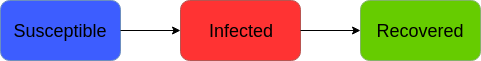
\includegraphics[width=.4\textwidth, angle=0]{./fig/fpabs/timedriven/SIR_transitions.png}
	\caption{States and transitions in the SIR compartment model.}
	\label{fig:sir_transitions}
\end{figure}

This model was also formalized using System Dynamics (SD) \cite{porter_industrial_1962}. In SD one models a system through differential equations, allowing to conveniently express continuous systems, which change over time, solving them by numerically integrating over time, which gives then rise to the dynamics. The SIR model is modelled using the following equation, with the dynamics shown in Figure \ref{fig:sir_sd_dynamics} .

\begin{equation}
\begin{aligned}
\frac{\mathrm d S}{\mathrm d t} = -infectionRate \\
\frac{\mathrm d I}{\mathrm d t} = infectionRate - recoveryRate \\
\frac{\mathrm d R}{\mathrm d t} = recoveryRate 
\end{aligned}
\end{equation}

\begin{equation}
\begin{aligned}
infectionRate = \frac{I \beta S \gamma}{N} \\
recoveryRate = \frac{I}{\delta} 
\end{aligned}
\end{equation}

\begin{figure}
	\centering
	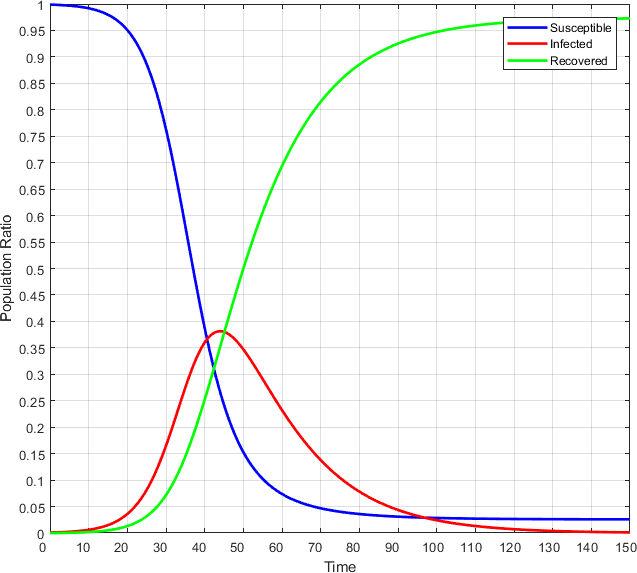
\includegraphics[width=0.5\textwidth, angle=0]{./fig/fpabs/timedriven/SIR_SD_1000agents_150t_001dt.png}
	\caption{Dynamics of the SIR compartment model using the System Dynamics approach. Population Size $N$ = 1,000, contact rate $\beta =  \frac{1}{5}$, infection probability $\gamma = 0.05$, illness duration $\delta = 15$ with initially 1 infected agent. Simulation run for 150 time-steps. Generated using our pure functional SD approach (see Chapter \ref{sub:generalising_system_dynamics}).}
	\label{fig:sir_sd_dynamics}
\end{figure}

The approach of mapping the SIR model to an ABS is to discretize the population and model each person in the population as an individual agent. The transitions between the states are happening due to discrete events caused both by interactions amongst the agents and time-outs. The major advantage of ABS is that it allows to incorporate spatiality as shown in Section \ref{sec:adding_env} and simulate heterogenity of population e.g. different sex, age. This is not possible with other simulation methods e.g. SD or Discrete Event Simulation \cite{zeigler_theory_2000}.

According to the model, every agent makes \textit{on average} contact with $\beta$ random other agents per time unit. In ABS we can only contact discrete agents thus we model this by generating a random event on average every $\frac{1}{\beta}$ time units. We need to sample from an exponential distribution because the rate is proportional to the size of the population \cite{borshchev_system_2004}. Note that an agent does not know the other agents' state when making contact with it, thus we need a mechanism in which agents reveal their state in which they are in \textit{at the moment of making contact}. This mechanism is an implementation detail, which we will derive in our implementation steps. For now we only assume that agents can make contact with each other somehow.

The \textit{parallel} strategy matches the semantics of the agent-based SIR model due to the underlying roots in the System Dynamics approach. As discussed already in Chapter \ref{sub:par_strategy}, in the parallel update-strategy, the agents act conceptually all at the same time in lock-step. This implies that they observe the same environment state during a time-step and actions of an agent
are only visible in the next time-step - they are isolated from each other. As will become apparent, FP can be used to enforce the correct application of this strategy already on the compile-time level.

\subsection{A pure functional implementation}
TODO: follow the PFE paper but add a few references back to the implementing ABS chapter so it is clear what problems we are currently solving. also might explain some concepts bit more in depth e.g. continuations?

As described in the Chapter \ref{sec:back_frp}, Arrowized FRP \cite{hughes_generalising_2000} is a way to implement systems  with continuous and discrete time-semantics where the central concept is the signal function, which can be understood as a process over time, mapping an input- to an output-signal. Technically speaking, a signal function is a continuation which allows to capture state using closures and hides away the $\Delta t$, which means that it is never exposed explicitly to the programmer, meaning it cannot be manipulated.

As already pointed out, agents need to perceive time, which means that the concept of processes over time is an ideal match for our agents and our system as a whole, thus we will implement them and the whole system as signal functions.

\subsection{Discussion}
Our FRP based approach is different from traditional approaches in the ABS community. First it builds on the already quite powerful FRP paradigm. Second, due to our continuous time approach, it forces one to think properly of time-semantics of the model and how small $\Delta t$ should be. Third it requires one to think about agent interactions in a new way instead of being just method-calls.

Because no part of the simulation runs in the IO Monad and we do not use \textit{unsafePerformIO} we can rule out a serious class of bugs caused by implicit data-dependencies and side-effects, which can occur in traditional imperative implementations.

Also we can statically guarantee the reproducibility of the simulation, which means that repeated runs with the same initial conditions are guaranteed to result in the same dynamics. Although we allow side-effects within agents, we restrict them to only the Random Monad in a controlled, deterministic way and never use the IO Monad, which guarantees the absence of non-deterministic side effects within the agents and other parts of the simulation.

Determinism is also ensured by fixing the $\Delta t$ and not making it dependent on the performance of e.g. a rendering-loop or other system-dependent sources of non-determinism as described by \cite{perez_testing_2017}. Also by using FRP we gain all the benefits from it and can use research on testing, debugging and exploring FRP systems \cite{perez_testing_2017, perez_back_2017}.

Also we showed how to implement the \textit{parallel} update-strategy \cite{thaler_art_2017} in a way that the correct semantics are enforced and guaranteed already at compile time through the types. This is not possible in traditional imperative implementations and poses another unique benefit over the use of functional programming in ABS.

The result of using FRP allows expressing continuous time-semantics in a very clear, compositional and declarative way, abstracting away the low-level details of time-stepping and progress of time within an agent.
	
Our approach can guarantee reproducibility already at compile time, which means that repeated runs of the simulation with the same initial conditions will always result in the same dynamics, something highly desirable in simulation in general. This can only be achieved through purity, which guarantees the absence of implicit side-effects, which allows to rule out non-deterministic influences at compile time through the strong static type system, something not possible with traditional object-oriented approaches. Further, through purity and the strong static type system, we can rule out important classes of run-time bugs e.g. related to dynamic typing, and the lack of implicit data-dependencies which are common in traditional imperative object-oriented approaches.
	
Using pure functional programming, we can enforce the correct semantics of agent execution through types where we demonstrate that this allows us to have both, sequential monadic behaviour, and agents acting \textit{conceptually} at the same time in lock-step, something not possible using traditional object-oriented approaches.

Currently, the performance of the system does not come close to imperative implementations. We compared the performance of our pure functional approach as presented in Section \ref{sec:adding_env} to an implementation in Java using the ABS library RePast \cite{north_complex_2013}. We ran the simulation until $t = 100$ on a 51x51 (2,601 agents) with $\Delta t = 0.1$ (unknown in RePast) and averaged 8 runs. The performance results make the lack of speed of our approach quite clear: the pure functional approach needs around 72.5 seconds whereas the Java RePast version just 10.8 seconds on our machine to arrive at $t = 100$. It must be mentioned, that RePast does implement an event-driven approach to ABS, which can be much more performant \cite{meyer_event-driven_2014} than a time-driven one as ours, so the comparison is not completely valid. Still, we have already started investigating speeding up performance through the use of Software Transactional Memory \cite{harris_composable_2005, harris_transactional_2006}, which is quite straight forward when using MSFs. It shows very good results but we have to leave the investigation and optimization of the performance aspect of our approach for further research as it is beyond the scope of this paper.

Despite the strengths and benefits we get by leveraging on FRP, there are errors that are not raised at compile time, e.g. we can still have infinite loops and run-time errors. This was for example investigated in \cite{sculthorpe_safe_2009} where the authors use dependent types to avoid some run-time errors in FRP. We suggest that one could go further and develop a domain specific type system for FRP that makes the FRP based ABS more predictable and that would support further mathematical analysis of its properties. Furthermore, moving to dependent types would pose a unique benefit over the traditional object-oriented approach and should allow us to express and guarantee even more properties at compile time. We leave this for further research.

In our pure functional approach, agent identity is not as clear as in traditional object-oriented programming, where there is a quite clear concept of object-identity through the encapsulation of data and methods. Signal functions don't offer this strong identity and one needs to build additional identity mechanisms on top e.g. when sending messages to specific agents.

We can conclude that the main difficulty of a pure functional approach evolves around the communication and interaction between agents, which is a direct consequence of the issue with agent identity. Agent interaction is straight-forward in object-oriented programming, where it is achieved using method-calls mutating the internal state of the agent, but that comes at the cost of a new class of bugs due to implicit data flow. In pure functional programming these data flows are explicit but our current approach of feeding back the states of all agents as inputs is not very general. We have added further mechanisms of agent interaction which we had to omit due to lack of space.

\subsection{Other approaches}
Sequential: see event-driven
Concurrent: see STM chapter
Actor: not discussed in this thesis but briefly 

\subsection{Super-Sampling}
when super-sampling is mentioned in the PFE paper extend it and add FrABS report, also show superSampling function implementation from PFE paper and FrABS with full body implementation

\chapter{Pure functional event-driven ABS}
\label{ch:eventdriven}

In this chapter we build on the previous discussion of update strategies in Chapter \ref{ch:impl_abs} and the implementation techniques presented in the time-driven approach of Chapter \ref{ch:timedriven} to develop concepts for event-driven ABS in a pure functional way. 

\medskip

In event-driven ABS \cite{meyer_event-driven_2014}, the simulation is advanced through events: agents and the environment schedule events into the future and react to incoming events scheduled by themselves, other agents, the environment or the simulation kernel. Time is discrete in this approach: it advances step-wise from event to event, where each event has an associated receiver and $\Delta t$, indicating the delay to the current virtual simulation time when should be scheduled. This implies that time could stay constant, for example when an event is scheduled with $\Delta t = 0$ the virtual simulation time does not advance. Further, agents can schedule events to themselves, emulating a recurring behaviour, which in turn emulates pro-active behaviour. Because agents can adopt and change their state and behaviour when processing an event, this means that even if time does not advance, agents can change. This non-signal behaviour is the fundamental difference to the time-driven approach in Chapter \ref{ch:timedriven}. Further, this mechanism is used to implement synchronous agent interactions pure functionally as discussed in the respective sections below.

The event-driven approach makes the simulation kernel technically closely related to a Discrete Event Simulation (DES) \cite{zeigler_theory_2000}. Due to the necessity of imposing a correct ordering of events in this type of ABS, it needs to be stepped event by event, with the \textit{sequential} update strategy, as introduced in Chapter \ref{sec:seq_strategy}. It is important to emphasise that only the semantics of the sequential update strategy allow the kind of features  presented in the following sections, as the agents act one after the other, seeing the effects of previous agents in the same time step. This would not make sense in the parallel update strategy as used in time-driven ABS, where agents act conceptually at the same time - event-driven ABS is inherently sequential due to its fundamental reliance on effects as will become clearer in the sections below. Note that there exists also Parallel DES (PDES) \cite{fujimoto_parallel_1990}, which processes events in parallel and deals with inconsistencies by reverting to consistent states. We hypothesise that a pure functional approach could be beneficial in such an approach due to persistent data structures and explicit handling of side effects but we leave this for further research.

\medskip

We start introducing the concepts of agent identity and event scheduling utilising both \textit{Reader} and \textit{Writer} Monads. We do this by using an event-driven agent-based SIR model, inspired by \cite{macal_agent-based_2010}. We then use the highly complex Sugarscape model as introduced in Chapter \ref{sec:sugarscape}, to develop more advanced features of ABS in a pure functional context: dynamic creation and removal of agents during simulation, adding a shared mutable environment, local mutable agent state and synchronous agent interactions. 
%Note that the Sugarscape model is not a real event-driven model like the event-driven SIR one is as in it the agents do schedule events but they don't do this into the future - events in Sugarscape don't have associated time-stamps.

\section{Basics of event-driven ABS}
\label{sec:eventdriven_basics}

In this section we derive the basics of event-driven ABS using the SIR model, as introduced in Chapter \ref{sec:sir_model}, with an event-driven approach inspired by \cite{macal_agent-based_2010}. Although it is a fundamentally different approach to ABS than the time-driven implementation in Chapter \ref{sec:timedriven_firststep} both solutions are quantitatively equal as they produce the same class of dynamics. Qualitatively they fundamentally differ though in terms of expressivity and performance as we will see in the discussion.

The basics of event-driven ABS are the concept of agent identity, events and event-scheduling. We introduce them step-by-step using various Monads and then generalise to a \textit{tagless final} approach, which has various benefits as pointed out in the respective section. 

\subsection{An event-driven SIR}
Before we can derive implementation concepts, we first need to discuss how an event-driven SIR model works, as inspired by \cite{macal_agent-based_2010}. Fundamentally, what is required is to transform all time-dependent behaviour and agent interactions into the scheduling and receiving of events. For the SIR this should be trivial and straightforward, taking inspiration from the time-driven implementation, where we simply translate the occurrences of events generated by \textit{occasionally} into scheduling of events. For agent interactions we also use events, making this more explicit than in the time-driven approach. As already pointed out, assuming that events have a receiver and a scheduling time given as $\Delta t$ relative to the current simulation time, we end up with three event-types:

\begin{enumerate}
	\item \textbf{MakeContact} - is used to let susceptible agents pro-actively make contact with $\beta$ (contact rate) other agents per 1 time-unit.
	\item \textbf{Contact$_{Sender, \ SIRState}$} - is used to make contact between agents where, agents reveal their state by sending or replying their current state.
	\item \textbf{Recover} - is used to let infected agents recover pro-actively after the given $\delta$ (illness duration). 
\end{enumerate}

Now we can give a concise definition of all three agent behaviours:

\paragraph{Susceptible Agent}
\begin{itemize}
	\item A susceptible agent initially schedules a \textit{MakeContact} event with $\Delta t = 1$ to itself.
	\item When receiving \textit{MakeContact}, the agent sends a \textit{Contact} event to $\beta$ (contact rate) random other agents with $\Delta t = 0$ and \textit{SIRState} of \textit{Susceptible}, resulting in these events to be scheduled immediately. Further, the agent schedules \textit{MakeContact} with $\Delta t = 1$ to itself, to keep the pro-active process of making contact with other agents active.
	\item When the agent receives a \textit{Contact} event, it checks if it is from an infected agent (\textit{SIRState} is \textit{Infected}). If the event is not from an infected agent, it ignores it, otherwise it becomes infected with a given probability.
\end{itemize}

\paragraph{Infected Agent}
\begin{itemize}
	\item An infected agent initially schedules a \textit{Recover} event to itself, with an exponentially distributed random $\Delta t$ of $\delta$ (illness duration).
	\item When the agent receives a \textit{Contact} event, it checks if it is from a susceptible agent (\textit{SIRState} is \textit{Susceptible}). If the event is not from a susceptible agent, it ignores it, otherwise it simply replies to this susceptible agent with a \textit{Contact} event with $\Delta t = 0$ and and \textit{SIRState} of \textit{Infected}.
\end{itemize}

\paragraph{Recovered Agent}
The recovered agent does not change any more, reacts to no incoming events and schedules no events - it stays constantly \textit{Recovered} forever.

\medskip

It is easy to see that this behaviour emulates the time-driven one and indeed in Figure \ref{fig:sir_eventdriven_dynamics} it is also visually clear that it produces similar dynamics. A striking difference are the small spikes and steps in the dynamics, which stem from the fact that time advances discretely and not continuous as in the time-driven implementation. In Chapter \ref{ch:sir_invariants}, we use property-based testing to show that both implementations indeed produce similar distributions in their dynamics, thus putting the claim that both implementations are quantitatively equal on a much more robust ground.

\begin{figure}
	\centering
	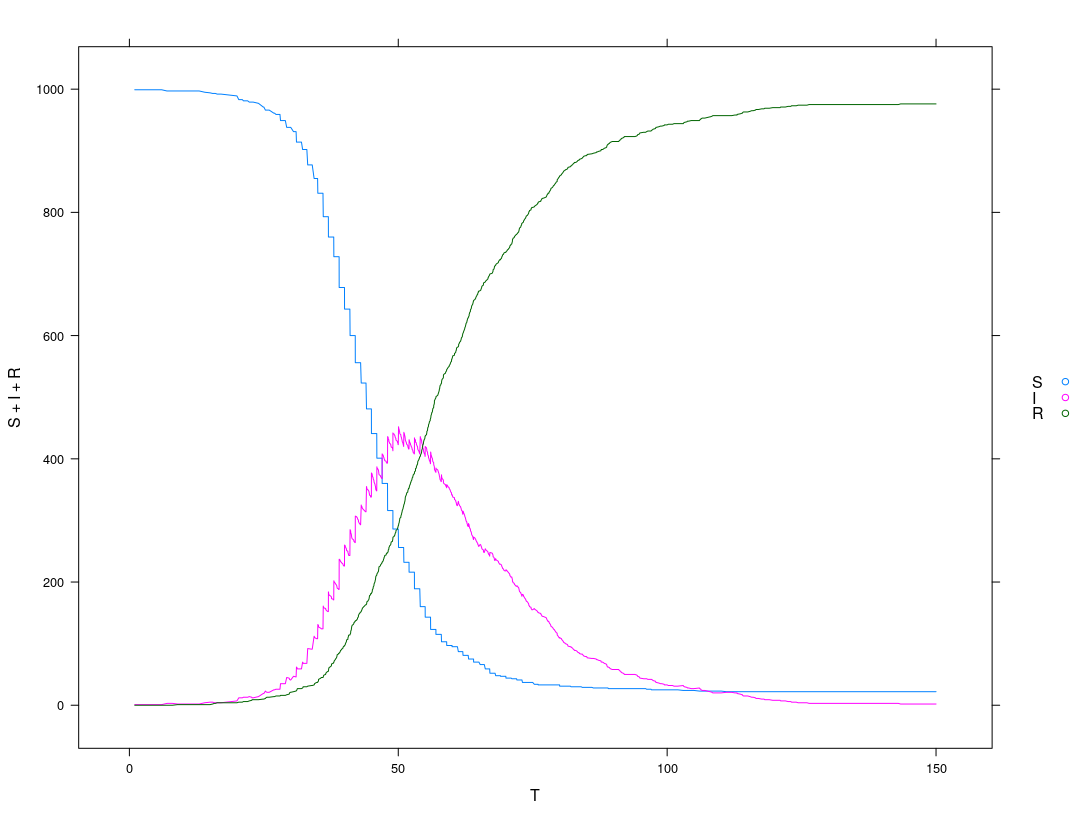
\includegraphics[width=0.7\textwidth, angle=0]{./fig/eventdriven/sir_eventdriven.png}
	\caption{Dynamics of the event-driven SIR model. Population Size $N$ = 1,000, contact rate $\beta = \frac{1}{5}$, infection probability $\gamma = 0.05$, illness duration $\delta = 15$ with initially 1 infected agent. Simulation run for 150 time-steps.}
	\label{fig:sir_eventdriven_dynamics}
\end{figure}

\subsection{Events, Agent Identity and Scheduling}
We can now start to discuss the concepts from an implementation perspective. First, we need to make the concept of an event explicit: they are of a given type, have a receiver and a time-stamp in \textit{absolute} simulation time when they shall be scheduled. We keep the event-type polymorphic and represent the receiver by an \textit{AgentId} which is a simple \textit{Int}. For efficient scheduling, the events are kept in a priority-queue \footnote{We are using the \textit{Data.PQueue.Min} implementation from the \textit{pqueue} package.}, sorted ascending by the time-stamp. Thus we define the following:

\begin{HaskellCode}
type Time        = Double
type AgentId     = Int
data QueueItem e = QueueItem e AgentId Time

-- the event priority-queue
type EventQueue e = PQ.MinQueue (QueueItem e)

-- implement Ord for QueueItem for acended sorting
instance Ord (QueueItem e) where
  compare (QueueItem _ _ t1) (QueueItem _ _ t2) = compare t1 t2
\end{HaskellCode}

Next, we define a polymorphic type for the agent. In event-driven ABS, due to the fact that agents are not signals any more, we abandon time-aware signal functions of BearRiver from the previous chapter and focus solely on Monadic Stream Functions (MSF). In event-driven ABS agents receive events, thus as input to an \textit{MSF} the polymorphic event type \textit{e} is used. As output, the polymorphic output type \textit{o} is used, which will be instantiated to a specific monomorphic type in the SIR model below. The question is now what Monad shall be used. For scheduling purposes (and because models might require it), agents should be able to \textit{read} the current simulation time: this is accomplished through a \textit{ReaderT Time}. Further, agents should be able to \textit{read} the identities of the other agents available in the simulation so they can schedule events to them when necessary: this is accomplished through a \textit{ReaderT [AgentId]}. Most importantly, agents have to be able to schedule events, meaning they have to be able to \textit{write} the events into some sink where they are accumulated for scheduling: this is accomplished through a \textit{WriterT [QueueItem e]}. Finally, the transformer stack needs to be extendible by other Monads, specified in concrete models like the SIR below, so we add another polymorphic type \textit{m}, indicating the closing Monad (stack).

\begin{HaskellCode}
type ABSMonad m e   = ReaderT Time (WriterT [QueueItem e] (ReaderT [AgentId] m))
type AgentMSF m e o = MSF (ABSMonad m e) e o
\end{HaskellCode}

Note that BearRivers \textit{SF} has also a \textit{ReaderT Double} as the innermost Monad but we deliberately avoided its use because the intended semantics of an \textit{SF} are different: the value in the \textit{ReaderT} of the \textit{SF} represents the sampling time-delta and not the absolute time, as in the event-driven case.

We can already implement a few polymorphic functions, operating on the given Monad stack. First, we implement a function \textit{allAgentIds} which simply returns the \textit{AgentId} of all agents, the contents of the \textit{ReaderT [AgentId]}. Second, we implement a function \textit{scheduleEvent} which allows to schedule a given event to a given receiver into the future given a specific time-delay, relative to the current simulation time.
 
\begin{HaskellCode}
allAgentIds :: Monad m => (ABSMonad m e) [AgentId]
allAgentIds = lift (lift ask)

scheduleEvent :: Monad m
              => e        -- ^ event
              -> AgentId  -- ^ receiver
              -> Double   -- ^ time-delay
              -> (ABSMonad m e) ()
scheduleEvent e aid dt = do
  -- get current simulation time
  t <- ask
  -- construct queue item
  let q = QueueItem e aid (t + dt)
  -- write/append (tell) to the WriterT (QueueItem e)
  lift (tell [q])
\end{HaskellCode}

Processing events can also be implemented generically and is straight forward, thus we only discuss the subtleties. For efficient lookup of event receivers all agents are organised into an \textit{IntMap}, which also holds the current output of the agent, to allow sampling of the domain-state. In general, the domain-state is highly model specific, thus a generic implementation needs to offer some mechanism to update the domain-state after an event, a process we named domain-state sampling. Our approach is to call a function which receives the agent map and returns a new domain-state for the current event/time-step. These domain-states are appended to an infinite list which forms the output of the simulation.

The events are then processed in the order provided by the queue and each event is executed with the given receiver. Running a receiver is simply achieved using the agent map, where a reviver is looked up and its \textit{MSF} is evaluated with the given event as input and the resulting monadic actions executed with the given information.
 
\subsection{Parametrising for SIR}
With the generic concepts now established, we show how to parametrise them to the concrete SIR model. First, we define the already well known states the agents can be in and the three different event types, as already introduced above.

\begin{HaskellCode}
data SIRState = Susceptible | Infected | Recovered
data SIREvent = MakeContact | Contact AgentId SIRState | Recover 
\end{HaskellCode}

Next, we parametrise the \textit{ABSMonad} to the SIR model: because behaviour is stochastic, we need to make use of the \textit{Rand} Monad, which also closes the Monad stack of \textit{ABSMonad}. Further, the event type is obviously parametrised to \textit{SIREvent}.

\begin{HaskellCode}
type SIRMonad g = ABSMonad (Rand g) SIREvent
\end{HaskellCode}

Now we define a \textit{SIRAgent} which can be understood as a constructing function, run once upon construction of the agent. This constructing functions runs in the \textit{SIRMonad}, thus agents can already make full use of the functionality, so they can schedule initial events, depending on their initial state. This is important for the susceptible and infected agent, which both need to schedule initial events for pro-active behaviour. The constructing functions also takes the \textit{AgentId} of the agent, thus making it available to the agent at construction time. It returns the initial agent-behaviour as \textit{AgentMSF}.

\begin{HaskellCode}
type SIRAgent g 
       = AgentId -> (SIRMonad g) (AgentMSF (SIRMonad g) SIREvent SIRState)
\end{HaskellCode}

The implementation of the constructing function of type \textit{SIRAgent} is straight forward and follows the specification given above. It makes use of the functions \textit{scheduleMakeContact} and \textit{scheduleRecovery} which are implemented using the generic \textit{scheduleEvent} from above.

\begin{HaskellCode}
sirAgent :: RandomGen g 
         => Int         -- ^ contact rate (beta)
         -> Double      -- ^ infectivity (gamma)
         -> Double      -- ^ illness duration (delta)
         -> SIRState    -- ^ initial state of the agent
         -> SIRAgent g
sirAgent beta gamma delta Susceptible aid = do
  -- on start, schedule MakeContact to itself
  scheduleMakeContact aid 1
  -- return susceptible behaviour
  return (susceptibleAgent aid beta gamma delta)
sirAgent _ _ delta Infected aid = do
  -- on start, schedule Recover to itself
  scheduleRecovery aid delta
  -- return infected behaviour
  return (infectedAgent aid)
sirAgent _ _ _ Recovered _ = 
  -- simply return recovered behaviour
  return recoveredAgent

scheduleMakeContact :: RandomGen g => AgentId -> Double -> (SIRMonadT g) ()
scheduleMakeContact aid = scheduleEvent MakeContact aid

scheduleRecovery :: RandomGen g => AgentId -> Double -> (SIRMonadT g) ()
scheduleRecovery aid delta = do
  dt <- (lift . lift . lift) (randomExpM (1 / delta))
  scheduleEvent Recover aid dt

-- returns random value following exponential distribution with given lambda
randomExpM :: MonadRandom m => Double -> m Double
\end{HaskellCode}

Now we are finally ready to implement the actual behaviour of an agent, where we discuss the full implementation of the susceptible agent behaviour. The basic structure should be already familiar from the time-driven approach, using \textit{switch} to dynamically change the behaviour to \textit{infectedAgent} in case of an infection. The behaviour is then a simple event handler, pattern matching on the incoming events:

\begin{HaskellCode}
susceptibleAgent :: RandomGen g 
                 => AgentId        -- ^ agents id
                 -> Int            -- ^ contact rate (beta)
                 -> Double         -- ^ infectivity (gamma)
                 -> Double         -- ^ illness duration (delta)
                 -> SIRAgentMSF g
susceptibleAgent aid beta gamma delta = 
    switch susceptibleAgentInfected (const (infectedAgent aid))
  where
    susceptibleAgentInfected :: RandomGen g 
                             => MSF (SIRMonadT g) SIREvent (SIRState, Maybe ()) 
    susceptibleAgentInfected = proc e -> do
      -- handle incoming event in monadic action
      ret <- arrM handleEvent -< e
      case ret of
        Nothing -> returnA -< (Susceptible, ret)
        _       -> returnA -< (Infected, ret)
\end{HaskellCode}

We strictly follow the specification as above. In case the agent receives \textit{Contact} from an infected agent it might become infected with a given probability. If it becomes infected, it schedules the recovery as it will make the transition to an infected agent.

\begin{HaskellCode}
-- received Contact from an Infected agent
handleEvent :: RandomGen g => SIREvent -> (SIRMonadT g) (Maybe ())
handleEvent (Contact _ Infected) = do
  -- become infected with gamma probability
  r <- (lift . lift . lift) (randomBoolM gamma)
  if r
    -- got infected 
    then do
      -- schedule Recovery to self, because switching to infected
      scheduleRecovery aid delta
      return (Just ())
    -- no infection
    else return Nothing

-- returns True with given probability
randomBoolM :: MonadRandom m => Double -> m Bool
\end{HaskellCode}

In case the agent receivers \textit{MakeContact} from itself, it will send \textit{Contact} with \textit{Susceptible} to $\beta$ (contact rate) other agents without delay and \textit{MakeContact} to itself with a delay of 1 time unit.

\begin{HaskellCode}
-- received MakeContact (from itself)
handleEvent MakeContact = do
  ais <- allAgentIds
  -- get beta random agents
  receivers <- (lift . lift . lift) (forM [1..beta] (const (randomElemM ais)))
  -- make contact with random agents
  mapM_ makeContactWith receivers
  -- re-schedule MakeContact to self
  scheduleMakeContact aid 1
  return Nothing
  
makeContactWith :: AgentId -> (SIRMonadT g) ()
makeContactWith receiver = 
  -- schedule Contact event immediately
  scheduleEvent (Contact aid Susceptible) receiver 0

-- picks an element randomly from the (non empty) list
randomElemM :: MonadRandom m => [e] -> m e
\end{HaskellCode}

The infected and recovered behaviours are conceptually equivalent and thus left as a trivial exercise to the reader. 

\subsection{Tagless Final}
At this point, the basics of event-driven ABS should be clear: how events are represented and processed using an event queue, how agents are represented with an \textit{MSF} and the idea behind the underlying polymorphic Monad transformer stack. Further, by parametrising the polymorphic concepts to the SIR model, we showed how to instantiate the generic concepts into a concrete model to arrive at a robust, maintainable and solid solution which is very likely to be correct up to the initial informal specification.

\medskip

In this section we briefly want to show how the so-called \textit{tagless final} approach \cite{kiselyov_typed_2012} can be used to arrive at a cleaner and more extensible interface of our implementation, which is also open to different \textit{interpretations}. The idea behind \textit{tagless final} is simple: specify the interface of operations in a typeclass and then write one or multiple interpreters for it, which simply means writing an instance implementation for the given typeclass. We start by defining the typeclass \textit{MonadAgent} with all the necessary methods, making up the effectful API of our agents. Note that we need to enable two language extensions: \textit{MultiParamTypeClasses} because we want to have more than a single type parameter in the typeclass - besides the Monad \textit{m}, we also want to parametrise over the event type \textit{e}; \textit{FunctionalDependencies} because the event type \textit{e} is determined by the Monad type \textit{m}.

\begin{HaskellCode}
{-# LANGUAGE MultiParamTypeClasses  #-}
{-# LANGUAGE FunctionalDependencies #-}

class Monad m => MonadAgent e m | m -> e where
  randomBool  :: Double -> m Bool
  randomExp   :: Double -> m Double
  randomElem  :: [a] -> m a
  getAgentIds :: m [AgentId]
  getTime     :: m Time
  getMyId     :: m AgentId
  schedEvent  :: e -> AgentId -> Double -> m ()
\end{HaskellCode}

The methods are self explaining. This typeclass is now used to replace the Monad stack by an overloaded type definition in the respective functions. Thus, the implementation of the agent constructing function and the agent behaviours are the same, with only the types changing slightly, lifts becoming obsolete and calls to function replaced by calls to methods of the typeclass. We don't give the full implementation again but only the type of the agent construction function as example, the types of the agent behaviours follow a similar pattern: 

\begin{HaskellCode}
sirAgent :: MonadAgent SIREvent m  -- CHANGED: overloaded with typeclass
         => Int         -- ^ contact rate (beta)
         -> Double      -- ^ infectivity (gamma)
         -> Double      -- ^ illness duration (delta)
         -> SIRState    -- ^ initial state of the agent
         -> m (MSF m SIREvent SIRState) -- CHANGED: no Monad stack
\end{HaskellCode}

Note that we added a \textit{getMyId} method, which shall return the \textit{AgentId} of the agent itself, avoiding the need for the agent of keeping the agent id around and also making it possible to implement more robust self-scheduling functions. For example, the \textit{scheduleRecovery} function is implemented in the \textit{tagless final} approach in the following way:

\begin{HaskellCode}
scheduleRecovery :: MonadAgent SIREvent m => Double -> m ()
scheduleRecovery delta = do
  -- draw random value from exponential distribution
  dt <- randomExp (1 / delta)
  -- get id of agent, no more need to pass it explicitly
  ai <- getMyId
  -- schedule Recover to itself
  schedEvent Recover ai dt
\end{HaskellCode}

What we are missing is a \textit{pure} interpreter for the agent implementation and the \textit{MonadAgent} typeclass. We start by defining a \textit{newtype}, which basically is a conceptually similar Monad stack as in the original implementation without the \textit{tagless final} approach. We let Haskell automatically derive monadic typeclasses, Functor, Applicative and Monad instances which saves a lot of boiler plate code, for which the \textit{GeneralizedNewtypeDeriving} language extension is required. Instead of the \textit{Rand} Monad, a \textit{StateT SimState} is used, which carries the random-number generator and other data  for synchronous agent interactions as will be discussed in the respective sections.

\begin{HaskellCode}
{-# LANGUAGE GeneralizedNewtypeDeriving #-}

newtype SIRAgentPure a = SIRAgentPure 
  { unSirAgentPure :: ReaderT (Time, AgentId, [AgentId]) -- combined into one
                        (WriterT [QueueItem SIREvent]
                          (State SimState)) a}
  deriving (Functor, Applicative, Monad, 
            MonadReader (Time, AgentId, [AgentId]),
            MonadWriter [QueueItem SIREvent],  
            MonadState SimState)
\end{HaskellCode}

Having this \textit{newtype} we can now write a \textit{pure} interpreter for the \textit{MonadAgent}. The implementations are straight forward and should be self explanatory. To run \textit{Rand} Monad actions, the function \textit{runRandWithSimState} is used, which extracts the random-number generator from \textit{SimState}, runs the action and puts the changed random-number generator back into the \textit{SimState}.

\begin{HaskellCode}   
{-# LANGUAGE FlexibleContexts           #-}
{-# LANGUAGE MultiParamTypeClasses      #-}
      
instance MonadAgent SIREvent SIRAgentPure where
  randomBool = runRandWithSimState . randomBoolM
  randomElem = runRandWithSimState . randomElemM
  randomExp  = runRandWithSimState . randomExpM
  -- schedEvent :: SIREvent -> AgentId -> Double -> m ()
  schedEvent e receiver dt = do
    t <- getTime 
    tell [QueueItem e receiver (t + dt)]
  -- getAgentIds :: m [AgentId]
  getAgentIds = asks trd
  -- getTime :: m Time
  getTime = asks fst3
  -- getMyId :: m AgentId
  getMyId = asks snd3

fst3 :: (a,b,c) -> a
snd3 :: (a,b,c) -> b
trd :: (a,b,c) -> c
runRandWithSimState :: MonadState SimState m => Rand StdGen a -> m a
\end{HaskellCode}

The main benefit of a \textit{tagless final} approach is that it is a solution to the expression problem \cite{kiselyov_typed_2012}: it is possible to add new interpreters of an embedded language and add new functionality without breaking the existing implementations. Interpretation in our case means that we can use different underlying Monads to run the agents: if we want to guarantee purity, no \textit{IO} Monad shall be used. Otherwise when concurrency with a lock-based approach or a lock-free approach is required \textit{IO} or \textit{STM} can be used in the underlying interpreter. Also, for reproducible unit testing, one can write custom test-interpreters where methods always return a-priori known results, similar to mocking. Adding new functionality is less an issue here but might become highly important when designing a more general ABS library, building on the \textit{tagless final} approach. It would allow the user of such a library to extend existing agents or default behaviour with new, custom-built methods, without breaking the existing ones. We leave that for further research.

\section{Advanced features}
\label{sec:advanced_eventdriven_ABS}

In the previous section we established the basics of event-driven ABS. It is now clear how events are represented, how agent identity is handled, how agents receive and schedule events, how events are scheduled and domain state is sampled. Furthermore, by using the \textit{tagless final} approach, we arrived at an elegant, extensible and robust solution, which separates specification, the agent and its behaviour, from its implementation, a \textit{pure} interpreter. 

In this section we present more advanced concepts of event-driven ABS, necessary in models with much higher complexity than the simple SIR. We developed these concepts using the Sugarscape model as introduced in Chapter \ref{sec:sugarscape}. Consequently we will discuss them from this model's perspective. More specifically, we show how to create and remove agents dynamically during simulation, add a shared mutable environment, model local mutable agent state and finally how synchronous agent interactions can be implemented. Together with the basics of event-driven ABS, with these concepts established it should be possible to implement a wide range of event-driven ABS models. For this we developed a full implementation of the Sugarscape model, in which we explored the concepts presented in this chapter, with the code accessible from the \href{https://github.com/thalerjonathan/haskell-sugarscape}{code repository}~\cite{thaler_sugarscape_repository}.

\input{./tex/research/eventdriven/advanced/sugarscape.tex}

\input{./tex/research/eventdriven/advanced/dynamic.tex}

\input{./tex/research/eventdriven/advanced/environment.tex}

\input{./tex/research/eventdriven/advanced/local.tex}

\input{./tex/research/eventdriven/advanced/interactions.tex}

%\section{Implementation Approaches}
5 Pages

This is now very programming-language specific

\begin{itemize}
	\item Mapping the strategies to 3 programming-languages: Java, Scala with Actors, Haskell
	\item Comparing the programming languages in regard of their suitability to implement each of these strategies
	\item Screen-shots of results of the same simulation-model with all the strategies
\end{itemize}

%\input{./tex/eventdriven/eventdrivenSIR.tex}

\section{Discussion}
Although there are similarities to the work of \cite{botta_time_2010} (the use of messages and the problem of when to advance time in models with arbitrary number synchronised agent-interactions), we approach our agents differently. First in our approach an agent is only a single MSF and thus can not be directly queried for its internal state / its id or outgoing messages, instead of taking a list of messages, our agents take a single event/message and can produce an arbitrary number of outgoing messages together with an observable state - note that this would allow to query the agent for its id and its state as well by simply sending a corresponding message to the agents MSF and requiring the agent to implement message handling for it. Also the state of our agents is \textit{completely} localised and there is no means of accessing the state from outside the agent, they are thus "fully encapsulated agents" \cite{botta_time_2010}. Note that the authors of \cite{botta_time_2010} define their agents with a polymorphic agent-state type \textit{s}, which implies that without knowledge of the specific type of \textit{s} there would be no way of accessing the state, rendering it in fact also fully encapsulated. The problem of advancing time in our approach is solved not exactly the same but conceptually it is the same: after sending a tick message to each agent (in random order), we process all agents until they are idle: there are no more enqueued messages / events in the queue.

our eventdriven approach makes heavy use of 2 state monads, thus one might ask what the benefits are, after all we seem to fall back into stateful, imperative style programming. we agree that our approach is just one way of implementing abs in fp but we think we have come a long way thus making our approach quite valuable even if there might be other approaches like shallow EDSLs. on the other hand even our stateful programming is highly restricted to only those 2 local datatypes which makes it much more manageable than unrestricted data mutation

quote carmack (\url{http://www.gamasutra.com/view/news/169296/Indepth_Functional_programming_in_C.php}): the main difficulty as a developer in software programming is to keep track of the states a program can be in and reason about them and their Validity

TODO: report LoC and compare it with other implementations we found on the internet

\section{Generalising}
TODO: can we derive an agent-monad?

TODO: what about comonads? read essence dataflow paper \cite{uustalu_essence_2006}: monads not capable of stream-based programming and arrows too general therefor comonads, we are using msfs for abs therefore streambased so maybe applicable to our approach/agents=comonads. comonads structure notions of context-dependent computation or streams, which ABS can be seen as of. this paper says that monads are not capable of doing stream functions, maybe this is the reason why i fail in my attempt of defining an ABS in idris because i always tried to implement a monad family. TODO: stopped at comonad section, continue from there. TODO understand comonads: https://www.schoolofhaskell.com/user/edwardk/cellular-automata and https://kukuruku.co/post/cellular-automata-using-comonads/

independent of time-driven or event-driven, our agents are MSFs.

\chapter*{} %Parallel pure functional ABS
\label{ch:parallel_abs}
TODO: we have looked into this also because we think our implementations are too slow and because pure FP is notoriously slow. This chapter can also be seen as an attempt on overcoming this problem 

Pure functional programming as in Haskell is well known and accepted as a remedy against the difficulties and problems of parallel computation \cite{hudak_history_2007}. The reason for it is clear: immutable data and explicit control of side-effects removes a large class of bugs due to data-conflicts, data-races. A fundamental benefit and strength of Haskell is, that it clearly distinguishes between parallelism and concurrency \textit{in its types} \cite{jones_tackling_2002}. It is very important for us to do so as well:

\begin{itemize}
	\item \textbf{Parallelism} - In parallelism, code runs in parallel solely for the purpose of doing more work within the same time, without interfering with other code through shared data (references, mutexes, semaphores,...). An example is the function \textit{map :: (a $\rightarrow$ b) $\rightarrow$ [a] $\rightarrow$ [b]}, which maps each element of type \textit{a} to \textit{b} using the function \textit{(a $\rightarrow$ b)}. It is a pure function and thus no sharing of data either through some monadic context or through the function \textit{(a $\rightarrow$ b)} is possible. This allows to run it in parallel: each function evaluation \textit{(a $\rightarrow$ b)} could potentially be executed at the same time, if we had enough CPU cures. Whether it runs actually in parallel or not, has no influence on the outcome, it is not subject to any non-deterministic influences. Thus we identify parallelism with pure and deterministic execution of data-transformations in parallel (data-parallelism).

	\item \textbf{Concurrency} - Concurrency refers to the decomposability property of a program, algorithm, or problem into order-independent or partially-ordered components or units \cite{lamport_time_1978}. Those parts \textit{can} be run in parallel which as a consequence \textit{might} give rise to asynchronous, non-deterministic events \footnote{Note that the functional \textit{concurrent} programming language Erlang \cite{armstrong_erlang_2010}, which uses the actor model for its concurrency model, was single-threaded from its conception in 1986 until around 2008. This might sound surprising but underlines the fact that concurrency per se has nothing to do with parallel execution.}.

	An example are two threads, running in parallel, which share data through a reference. Depending on the scheduling and the code which is run in each thread, this gives rise to very different access patterns - the events - to the shared data, with the potential for race conditions and dirty reads. In concurrency per definition, ordering is important and the challenge of implementing parallel, concurrent programs, is to write the program in a way that despite of these non-deterministic events it is still a correctly working program. Thus we identify concurrency with parallel, impure, non-deterministic execution of imperative-style and ordered monadic evaluation.
\end{itemize}

In the next two chapters we investigate the application of both parallelism and concurrency to our pure functional ABS approach. In general, we want to see if and how parallel and concurrent programming in Haskell is transferable to pure functional ABS and what the benefits are. In particular we are interested in speeding up the existing implementations by generally developing techniques that allow us to  \textit{run agents in parallel \footnote{Note that we use the term \textit{parallel} to identify both \textit{parallelism} and \textit{concurrency} and we distinguish between them whenever necessary using their respective terms.}}. 

Note that the focus here is primarily on the conceptual nature of how to apply parallelism and concurrency to pure functional ABS, thus we refrain from doing in-depth performance analysis up-front as it is beyond the scope of this work. Still, we are very well aware that mindlessly trying to apply parallel computation can actually result in loss of performance as a problem can only be sped up in so far as we can partition it and run those partitions in parallel. Further, parallel computation comes with an overhead and if the partitioning is too fine-grained, this overhead might eat up the speed up or make it even worse. Thus, in real-world problems, performance measurements have to come first, then one can investigate where and why the performance is lost. Only if this is properly understood one can decide whether parallelism or concurrency is applicable - or none at all because the problem is actually completely sequential. As D. Knuth famously put it: \textit{"Premature optimisation is the root of all evil"}, thus, when we see adding parallel computation as one way of optimising a problem, we need hard facts instead of wild guesses.

Besides performance improvement, we are generally interested in the implications of the way Haskell deals with parallelism and concurrency in its types. In particular we ask about the ability of keeping deterministic guarantees about the reproducibility of our simulations. We hypothesize that parallelism will allow us to retain \textit{all} static guarantees about reproducibility \textit{and} gives us a noticeable speed up. Further we hypothesize, that in concurrency we might see a bigger speed up but sacrifice the very guarantee about reproducibility. However, we assume that by using Haskell's unique approach to Software Transactional Memory (STM), we don't lose this guarantee completely - it will just get weakened by guaranteeing that the non-deterministic influence is through concurrency only \textit{and nothing else}.

\chapter{Parallelism in ABS}
The promise of parallelism in Haskell is compelling: speeding up the execution but retaining all static compile-time guarantees about determinism. In other words, using parallelism could give us a substantial performance improvement without sacrificing the static guarantees of reproducible outputs from repeated runs with initial conditions.

Generally, parallelism can be applied whenever the execution of code is order-independent, that is referential transparent, and has no implicit or explicit side-effects. In this section we introduce the two most important parallelism concepts of Haskell, \textit{evaluation} and \textit{data-flow} parallelism, and discuss their potential use in pure functional ABS in general. We follow \cite{marlow_parallel_2013} and refer to it for an in-depth discussion. Further, we show how these concepts can be added to our previously discussed use-cases of Chapters \ref{sec:timedriven_firststep}, \ref{sec:adding_env} and Sugarscape \ref{sec:eventdriven_implementation} and compare their performance over the original sequential approaches.

\section{Evaluation Parallelism}
Evaluation parallelism introduces so called strategies to evaluate lazy data-structures in parallel. Examples are strategies to evaluate a list, or tuples in parallel where for each element a spark is created. The fundamental concept Haskell uses to achieve evaluation parallelism is its own non-strictness nature. Non-strictness means that expressions are not eagerly evaluated when defined, like in imperative programming languages but only evaluated when their result is actually needed. This is implemented internally using thunks, which are pointers to expressions. When the value of an expression is needed, this thunk is accessed and the expression is reduced until the next constructor or lambda is encountered. This is called Weak Head Normal Form (WHNF) evaluation because it only reduces the "head" of the expression, which could consist of sub expressions. This indirection, the separation of data creation from consumption / evaluation, indeed enables evaluation parallelism and Haskell provides two additional functions to support this:

\begin{itemize}
	\item \textit{par :: a $\rightarrow$ b $\rightarrow$ b} Returns the second argument \textit{b} but evaluates the first argument \textit{a} in parallel. It is used when the result of evaluating \textit{a} is required later.
	
	\item \textit{seq :: a $\rightarrow$ b $\rightarrow$ b} - Returns the second argument \textit{b} but is strict in its first argument, which means it forces its evaluation to WHNF. It is used when the result of evaluating \textit{a} is required now.
\end{itemize}

Internally, evaluation parallelism is handled through so called \textit{sparks}, which are basically thunks which get evaluated in parallel. The Haskell runtime system manages sparks and distributes them to threads where they get executed. Due to their extremely light-weight nature, it is no problem to create tens of thousands of sparks. One has to bear in mind that even though evaluating in parallel through sparks is extremely cheap, it still has some overhead. Thus, the work-load of each element in a list might be too low for a spark, then one can distribute chunks of a list onto a single spark.
It is important to understand, that all this works without side-effects - the strategy combinators are all pure functions building on \textit{par} and \textit{seq}. This allows us to add parallelism to an algorithm by applying a parallel evaluation strategy to its result which e.g. is a lazy list - again this is possible through non-strictness, which separates the construction of data from its consumption.

\subsection{Evaluation Parallelism In ABS}
Using compositional parallelism is exactly what we use to aim at adding evaluation parallelism for agent execution in the non-monadic SIR example \ref{sec:timedriven_firststep}. We know that the whole simulation is a completely pure computation because Yampa is non-monadic, thus it is guaranteed that there are no side-effects - thus agents are run conceptually in parallel e.g. using map. Now we should be able to add parallelism without needing to re-implement \textit{dpSwitch} which is the function which runs the agents in parallel (Also re-implementing switch functions would not get us very far because of WHNF evaluation it is the wrong end to start parallel evaluation: probably only the arguments would be evaluated but not the agent behaviour.)

The solution is to add evaluation parallelism in the agent-output collection phase: where the recursive switch into the \textit{stepSimulation} function happens. There we use a evaluation strategy to evaluate the outputs of all agents in parallel. The agents will then be evaluated in parallel due to compositional parallelism, when we force the output of each in parallel. We give more details in the short case-study \ref{parallel_nonmonadic_sir} below.

TODO: can we apply it to monadic SIR ? hypothesis is that yes we can apply it but we wont see any performance improvement because the sequential monadic code forces evaluation
TODO: we can use it to e.g map over a lazy data structure representing the environment - we show in the case-study if this is applicable to the sugarscape


\section{Data-flow parallelism}
TODO: cite A Monad for Deterministic Parallelism Marlow paper
When relying on a lazy data structure to apply parallelism is not an option, evaluation strategies as presented before are not applicable. Further, although lazy evaluation brings compositional parallelism, it makes it hard to reason about performance. Data-flow parallelism offers an alternative over evaluation strategies, where the programmer can give more details but gains more control: data dependencies are made explicit and reliance on lazy evaluation is avoided.
Data-flow parallelism is implemented through the \textit{Par} Monad, which provides combinators for expressing data-flows: in this monad it is possible to \textit{fork} parallel tasks which communicate with each other through shared locations, so called \textit{IVar}s. Internally these tasks are scheduled by a work-stealing scheduler which distributes the work evenly on available processors at runtime. \textit{IVars} behave like futures or promises: they are initially empty and can be written once. Reading from an empty \textit{IVar} will cause the calling task (or main thread) to wait until it is filled. An example is a parallel evaluation of two fibonacci numbers:

\begin{HaskellCode}
runPar (do
  i <- new             -- create new IVar
  j <- new             -- create new IVar
  fork (put i (fib n)) -- fork new task compute fib n and put result into IVar i
  fork (put j (fib m)) -- fork new task compute fib m and put result into IVar j
  a <- get i           -- wait for the result from IVar i and collect it
  b <- get j           -- wait for the result from IVar j and collect it
  return (a,b)         -- return the sum
\end{HaskellCode}

Note that with this it is also possible to express parallel evaluation of a list or a tuple as with evaluation strategies. The difference though is, that it does avoid lazy evaluation. More importantly, putting a value into an \textit{IVar} requires the type of the value to have an instance of the \textit{NFData} typeclass. This simply means that a value of this type can be fully evaluated, not just to WHNF but to evaluate the full expression the value represents.

\subsection{Data-flow parallelism in ABS}
The Par monad seems to be a very suitable mechanism to enable agents to express data-flow parallelism within their behaviour. This is only possible with the monadic ABS approach as in the SIR implementation of Chatper TODO and the Sugarscape. An important fact is that if the Par monad is used, it has to be the innermost monad because it cannot be a transformer. This is emphasised by the fact that there exists no ParT transformer instance, like for other monads (e.g. StateT, RandT, ReaderT,... we used in the Sugarscape chapter). Making the Par monad a transformer would have (probably) the meaning of running the \textit{bind} in parallel. It is quite clear that this simply makes no sense: \textit{bind} is a function for composing / sequencing monadic actions, which in general involves side-effects of some kind. Side-effects inherently impose some sequencing where evaluation of different sequences has different meanings in general - thus the sequential nature of \textit{bind}. Thus follows that running monadic code in parallel is simply not possible in general due to side-effects \footnote{Besides, it would be not very clear what we are running in parallel within the \textit{bind} operator as there is nothing to parallelise in general e.g. no structure over which we can parallelise in general.} and thus there is no (meaningful) way to put the Par into a transformer stack.

% IGNORE FOR NOW
%\subsection{Data-structure parallelism}
%An environment could be organised and accessed through such a data-structure, which could potentially lead to big speed ups. Agents could locally read the data-structure data-parallel and the simulation kernel could feed the output of the agents data-parallel back into this structure.
%
%%https://learning.oreilly.com/library/view/parallel-and-concurrent/9781449335939/ch05.html
%
%general solution we opt for is  to run agents in parallel in our approaches. in other abs models we could apply data-structure parallelism and/or data-flow parallelism with huge Performance potential but thats always highly model dependent thus we dont go in depth here
\section{Case-Studies}
In this section we go a little bit more into detail how to apply the parallelism concepts as already outline above to our use-cases from Chapters \ref{sec:timedriven_firststep}, \ref{sec:adding_env} and Sugarscape \ref{sec:advanced_eventdriven_ABS}. We briefly demonstrate the technical details and refer to the full code in footnotes. Note that all timings are rough averages over multiple runs and not precise measurements because that is not the point here. We are only interested in showing what rough potential there is for speeding up computation through deterministic parallelism - we are not interested in high performance computation here but rather in conceptual comparisons between sequential and parallel implementations.

\input{./tex/parallelabs/parallelism/nonmonadic.tex}

\input{./tex/parallelabs/parallelism/monadic.tex}
\\
\input{./tex/parallelabs/parallelism/sugarscape.tex}

\section{Parallel Runs}
Often one needs to perform a large number of runs of the same simulation. The most prominent use-cases for this are:

\begin{itemize}
	\item Parameter Sweeps / Variations - to explore the parameter space and the dynamics under varying parameter configurations, the same simulation is run with varying parameters and the results recorded for statistical analysis.
	
	\item Stochastic replications - due to ABS stochastic nature, running a simulation only once does not allow to generalise or predict overall behaviour - one might have just hit an (un)fortunate special case. To counter this problem, in ABS multiple replications of the  simulation are run with same initial model parameters but with different random-number streams. All the results are collected and analysed stochastically (averaged, median,...) from which then more general properties can be derived.
\end{itemize}

In each case thousands of runs of the same simulation with different model parameters and / or varying random-number streams are needed, requiring a considerable amount of computing power.

Parallelism is a remedy to this problem because in each of these cases individual runs do not interfere with each other and thus can be seen as isolated from each other, like referential transparent, pure computations. Our approaches shown in Part II make this very explicit: the top level functions can always be made pure computations because we are ruling out \textit{IO} and thus even though Monads are employed in many cases, they are still pure. A benefit of our approach is that it is guaranteed at compile time, that individual runs do not interfere with each other and thus there is no danger that parallel runs influence each other. 

All this allows to implement parameter sweeps and stochastic replications both through evaluation and data-flow parallelism making another very compelling use-case - probably the most striking one - for the use of parallelism in ABS. We hypothesize that data-flow parallelism is better suited for this task because it makes parallelism more explicit as it is indeed a data-flow problem: we pass parameters to single replications which are run and return their results. To apply this we simply run the top level replication logic in the \textit{Par} Monad where replications are run in parallel by forking tasks and results are handed back through \textit{IVars}. If we want the convenience of having a monadic random-number generator within the \textit{Par} Monad, one can use the combined \textit{ParRand} Monad which provides both.

\subsection{Reflection}
Despite high hopes, there were very few opportunities to apply parallelism to our pure functional ABS. This has three reasons: it is often highly model specific and our models simply didn't offer a lot of suitable parallelisations, the data-structures have to support parallelism e.g. map doesn't, but we also have to say that the sequential nature of ABS in general seems to be less suited to parallelism. We will see that concurrency offers a remedy against that.

the difficulties / low ausbeute von parallelism just Shows how difficult it is to parallelise abs. also maybe our approach is not very well.suited e.g. not very functional?

In general we aimed at running agents in parallel using the various techniques. Because of the quite sequential nature of the agent behaviours themselves, there is much less potential for parallelism \textit{within} an agent, thus the obvious idea was to run them all in parallel because they are an obvious unit of partitioning, have considerable workload and can indeed be run in parallel under given circumstances.
Unfortunately it is not possible applying parallelism in case the agents run within a monadic context: we have side-effects which imposes ordering e.g. in the case of a

It becomes apparent, that applying parallelism to our approaches doesn't lead to very much performance increase. This is because in the cases were we can actually run the agents with evaluation parallelism, the performance is not bound by them. As soon as we switch to monadic agents, evaluation parallelism is out of the window, as agents can't be run in parallel anymore because side-effects require to impose a sequential ordering. This can be only tackled using non-deterministic concurrency, which we will show in-depth in the next chapter because it is much more promising than prallelism in terms of performance gain. Further it is also more technically involved and the way we chose to approach it using Software Transactional Memory (STM) hasn't been undertaken in this form ever and to our best knowledge we are the first one to do so.

We see a direct consequence of this that types also reflect the semantics of our model: when our agents are pure they can be run indeed in parallel and independent from each other, if they are monadic, then this is not applicable to parallelism. In the next section, we show how to approach this problem and come up with a solution where we can run monadic agents in parallel. This is obviously only possible within a concurrent setting which means we have to sacrifice determinism in our solution. Still we reach considerable speed ups using Software Transactional Memory.

We didn't discuss data parallelism on large array structure or parallelism on GPU as they are used in massively large numerical computation. These techniques achieve tremendous speed ups but are not applicable to ABS in general but only in model specific cases where e.g. each agent needs to crunch through arrays of numbers to perform numerical computations. We refer to \cite{marlow_parallel_2013} for a more in-depth discussion of both in Haskell and leave the application to pure functional ABS for further research.

\chapter{Concurrent ABS}
\label{ch:concurrent_abs}

%- no comparison to io or repast: the story is "concurrency with compile time guarantees", only mention that an io based single lock performs much worse in sir and slightly worse in sugarscape. leave Array i IORef for further research

In an ideal world, we would like to solve all our problems using parallelism but unfortunately, it can't be applied to all parallel problems and ABS is no exception. As soon as there are data-dependencies, like we have them in the Sugarscape model in the form of the read/write environment and synchronous agent-interactions, and to a lesser extent in the monadic SIR with the \textit{Rand} Monad, we cannot avoid concurrency. More general, this is due to the fact that agents are executed within a monadic context, from which the  sequencing of effectful computations immediately follows - this is the very meaning of the Monad abstraction. Indeed, we have shown both by argument and measurement in the previous chapter the very fact that parallelism is simply not applicable to monadic execution of agents due to sequencing of effects, which renders all attempts of running monadic agents in parallel void. In this chapter we discuss the use of concurrency to run agents which have a monadic context in parallel - which is the only way we can execute monadic agents at the same time.

\medskip

Traditional approaches to concurrency follow a lock-based approach, where sections which access shared data are synchronised through synchronisation primitives like mutexes, semaphores, monitors,... The lock-based path is a well trodden one, with all problems and benefits well established. In this chapter we follow a different path and look into using Software Transactional Memory (STM) for implementing concurrent ABS, which promises to overcome the problems of lock-based approaches. Although STM exists in other languages as well, Haskell was one of the first to natively build it into its core, thus it is a natural choice to follow that direction when already investigating pure functional ABS.

Unfortunately, as soon as we employ concurrency, we lose all static guarantees about reproducibility and the use of STM is no exception. Still, STM has the unique benefit that it can guarantee the lack of persistent side-effects at compile time, allowing unproblematic retries of transactions, something of fundamental importance in STM as will be described below. This implies also another \textit{very} compelling advantage of STM over unrestricted lock-based approaches: by using STM, we can reduce the side-effects allowed substantially and guarantee at compile time, that the differences between runs of same initial conditions will only stem from the fact that we run the simulation concurrently - \textit{and from nothing else}. All this makes the use of STM very compelling and to our best knowledge we are the very first to investigate the use of STM for implementing concurrent ABS in a systematic way.

\medskip

The paper \cite{discolo_lock_2006} gives a good indication how difficult and complex constructing a correct concurrent program is and shows how much easier, concise and less error-prone an STM implementation is over traditional locking with mutexes and semaphores. More important, it shows that STM consistently outperforms the lock-based implementations. We follow this work and compare the performance of lock-based and STM implementations and hypothesise that the reduced complexity and increased performance will be directly applicable to ABS as well.

We present two case studies using the already introduced SIR (Chapter \ref{sec:sir_model}) and Sugarscape (Chapter \ref{sec:sugarscape}) models. We compare the performance of lock-based and STM implementations in each case where we investigate both the scaling performance under increasing number of CPUs and agents. We show that the STM implementations consistently outperform the lock-based ones and scale much better to increasing number of CPUs both on local machines and on Amazon Cloud Services.

%Note that there exists also the actor model of concurrency, which is especially well suited to implement concurrent applications in functional languages. We give a short overview over it, existing research and its use in ABS in the section \ref{sec:actors} but leave it for further research as it has very different implications, which are beyond the focus of this thesis.

\section{Software Transactional Memory}
Software Transactional Memory was introduced by \cite{shavit_software_1995} in 1995 as an alternative to lock-based synchronisation in concurrent programming which, in general, is notoriously difficult to get right. This is because reasoning about the interactions of multiple concurrently running threads and low level operational details of synchronisation primitives is \textit{very hard}. The main problems are \cite{marlow_parallel_2013}:

\begin{itemize}
	\item Race conditions due to forgotten locks;
	\item Deadlocks resulting from inconsistent lock ordering;
	\item Corruption caused by uncaught exceptions;
	\item Lost wake-ups induced by omitted notifications.
\end{itemize}

What is worse, concurrency does not compose. It is very difficult to write two functions (or methods in an object) acting on concurrent data which can be composed into a larger concurrent behaviour. The reason for the difficulty is that one has to know about the internal details of locking, which breaks encapsulation and makes composition dependent on knowledge about their implementation. Therefore, it is impossible to compose two functions where, for example, one withdraws some amount of money from an account and the other deposits this amount of money into a different account. The problem is that one ends up with a temporary state where the money is in neither of the accounts, creating an inconsistency and a potential source for errors because threads can be rescheduled at any time.

STM promises to solve all of these problems for a low cost by executing actions \textit{atomically}, where modifications made in such an action are invisible to other threads and changes by other threads are also invisible until actions are committed - STM actions are atomic and isolated. When an STM action exits, either one of two outcomes happen: if no other thread has modified the same data as the thread running the STM action, then the modifications performed by the action will be committed and become visible to the other threads. If other threads have modified the data then the modifications will be discarded, the action rolled back and automatically restarted.

\subsection{Software Transactional Memory in Haskell}
The work of \cite{harris_composable_2005, harris_transactional_2006} added STM to Haskell, which was one of the first programming languages to incorporate STM with composable operations into its main core. In the Haskell implementation, STM actions run within the \texttt{STM} Monad. This restricts the operations to only STM primitives as shown below. This means that \texttt{STM} actions are always repeatable without persistent side effects because such persistent side effects (for example writing to a file, launching a missile) are not possible in the \texttt{STM} Monad. This is also the fundamental difference to \texttt{IO}, where all bets are off and \textit{everything} is possible because \texttt{IO} can run everything without restrictions.

Thus, the ability to \textit{restart} an action without any persistent effects is only possible due to the nature of Haskell's type system and by restricting the effects to \texttt{STM} only, ensures that only controlled effects, which can be rolled back, occur.

STM comes with a number of primitives to share transactional data. Amongst others the most important ones are:

\begin{itemize}
	\item \texttt{TVar} - a transactional variable which can be read and written arbitrarily;
	
	\item \texttt{TMVar} - a transactional \textit{synchronising} variable which is either empty or full. To read from an empty or write to a full \texttt{TMVar} will cause the current thread to block and retry its transaction when \textit{any} transactional primitive of this action has changed.
	
	\item \texttt{TArray} - a transactional array where each cell is an individual transactional variable \texttt{TVar}, allowing more finer-grained transactions instead of having the whole array in a \texttt{TVar}.
	
	\item \texttt{TChan} - a transactional channel, representing an unbounded FIFO channel, based on a linked list of \texttt{TVar}.
\end{itemize}

Furthermore STM also provides combinators to deal with blocking and composition:

\begin{itemize}
	\item \texttt{retry :: STM ()} retries an \texttt{STM} action. This will cause to abort the current transaction and block the thread it is running in. When \textit{any} of the transactional data primitives have changed, the action will be run again. This is useful to await the arrival of data in a \texttt{TVar}, or put more general, to block on arbitrary conditions. 
	
	\item \texttt{orElse :: STM a $\rightarrow$ STM a $\rightarrow$ STM a} allows us to combine two blocking actions where either one is executed, but not both. The first action is run and if it is successful its result is returned. If it retries, then the second is run and if that one is successful its result is returned. If the second one retries, the whole \texttt{orElse} retries. This can be used to implement alternatives in blocking conditions, which can obviously be nested arbitrarily.
\end{itemize}

To run an \texttt{STM} action the function \texttt{atomically :: STM a $\rightarrow$ IO a} is provided, which performs a series of \texttt{STM} actions atomically within the \texttt{IO} Monad. It takes the \texttt{STM} action, which returns a value of type \texttt{a} and returns an \texttt{IO} action which returns a value of type \texttt{a}. The \texttt{IO} action then can only be executed from within the \texttt{IO} Monad, either within the main thread or an explicitly forked thread.

STM in Haskell is implemented using optimistic synchronisation, which means that instead of locking access to shared data, each thread keeps a transaction log for each read and write to shared data that it makes. When the transaction exits, the thread checks whether it has a consistent view to the shared data or not. It checks whether other threads have written to memory it has read, thus it can identify whether a rollback is required or not.

However, STM does not come without issues. The authors of \cite{perfumo_limits_2008} analyse several Haskell STM programs with respect to their transactional behaviour. They identified the roll-back rate as one of the key metrics, which determines the scalability of an application. Although STM might promise better performance, they also warn of the overhead it introduces, which could be quite substantial in particular for programs which do not perform much work inside transactions as their commit overhead is high.

\subsection{STM Examples}
We provide two examples to demonstrate the use and semantics of STM. The first example is an implementation of the aforementioned functionality, where money is withdrawn from one account and transferred to another. The implementing function \texttt{transferFunds} takes two \texttt{TVar}, holding the account balances, and the amount to exchange. It executes using \texttt{atomically}, therefore running in the \texttt{IO} Monad. It uses the two functions \texttt{withdraw} and \texttt{deposit} which do the work of withdrawing some amount from one account and depositing some amount to another. This example demonstrates how easily STM can be used: the implementation looks quite straightforward, simply swapping values, without any locking involved or special handling of concurrency, other than the use of \texttt{atomically}.

\begin{HaskellCode}
transferFunds :: TVar Integer -> TVar Integer -> Integer -> IO ()
transferFunds from to n = atomically (do
  withdraw from n
  deposit to n)
  
withdraw :: TVar Integer -> Integer -> STM ()
withdraw account amount = do
  balance <- readTVar account
  writeTVar (balance - amount)
  
deposit :: TVar Integer -> Integer -> STM ()
deposit account amount = do
  balance <- readTVar account
  writeTVar (balance + amount)
\end{HaskellCode}

In the second example we show the retry semantics of STM, by using it within a \texttt{StateT} transformer where \texttt{STM} is the innermost Monad. It is important to understand that \texttt{STM} does not provide a transformer instance for very good reasons. If it would provide a transformer then we could make \texttt{IO} the innermost Monad and perform \texttt{IO} actions within \texttt{STM}. This would violate the retry semantics, as in case of a retry, \texttt{STM} is unable to undo the effects of \texttt{IO} actions in general. This stems from the fact that the \texttt{IO} type is simply too powerful and we cannot distinguish between different kinds of \texttt{IO} actions in the type, be it simply reading from a file or actually launching a missile. Let's look at the example code:

\begin{HaskellCode}
stmAction :: TVar Int -> StateT Int STM Int 
stmAction v = do
  -- print a debug output and increment the value in StateT 
  Debug.trace "increment!" (modify (+1))
  -- read from the TVar
  n <- lift (readTVar v)
  -- await a condition: content of the TVar >= 42
  if n < 42
    -- condition not met: retry
    then lift retry
    -- condition met: return content ot TVar
    else return n
\end{HaskellCode}

In this example, the \texttt{STM} is the innermost Monad in a stack with a \texttt{StateT} transformer. When \texttt{stmAction} is run, it prints an \texttt{'increment!'} debug message to the console and increments the value in the \texttt{StateT} transformer. Then it awaits a condition. For as long as \texttt{TVar} is less then 42 the action will retry whenever it is run. If the condition is met, it will return the content of the \texttt{TVar}. We see the combined effects of using the transformer stack where we have both the \texttt{StateT} and the \texttt{STM} effects available. The question is how this code behaves if we actually run it. To do this we need to spawn a thread:

\begin{HaskellCode}
stmThread :: TVar Int -> IO ()
stmThread v = do
  -- the initial state of the StateT transformer
  let s = 0
  -- run the state transformer with initial value of s (0)
  let ret = runStateT (stmAction v) s
  -- atomically run the STM block
  (a, s') <- atomically ret
  -- print final result
  putStrLn("final StateT state     = " ++ show s' ++
           ", STM computation result = " ++ show a)
\end{HaskellCode}

The thread simply runs the \texttt{StateT} transformer layer with the initial value of 0 and then the \texttt{STM} computation through \texttt{atomically} and prints the result to the console. The value of \texttt{a} is the result of \texttt{stmAction} and \texttt{s'} is the final state of the \texttt{StateT} computation. To actually run this example we need the main thread to update the \texttt{TVar} until the condition is met within \texttt{stmAction}:

\begin{HaskellCode}
main :: IO ()
main = do
  -- create a new TVar with initial value of 0
  v <- newTVarIO 0 
  -- start the stmThread and pass the TVar
  forkIO (stmThread v)
  -- do 42 times...
  forM_ [1..42] (\i -> do
    -- use delay to 'make sure' that a retry is happening for ever increment
    threadDelay 10000
    -- write new value to TVar using atomically
    atomically (writeTVar v i))
\end{HaskellCode}

If we run this program, we will see \texttt{'increment!'} printed 43 times, followed by \texttt{'final StateT state = 1, STM computation result = 42'}. This clearly demonstrates the retry semantics where \texttt{stmAction} is retried 42 times and thus prints \texttt{'increment!'} 43 times to the console. The \texttt{StateT} computation, however, is carried out only once and is always rolled back when a retry is happening. The rollback is easily possible in pure functional programming due to persistent data structure, by simply throwing away the new value and retrying with the original value. This example also demonstrates that any \texttt{IO} actions which happen within an \texttt{STM} action are persistent and can obviously not be rolled back. \texttt{Debug.trace} is an \texttt{IO} action masked as pure using \texttt{unsafePerformIO}.

\section{Software Transactional Memory in ABS}
\label{sec:stm_abs}
In this section we give a short overview of how we apply STM to pure functional ABS. In both case studies we fundamentally follow a time-driven, parallel approach as introduced in Chapter \ref{sub:par_strategy}, where the simulation is advanced by a given $\Delta t$ and in each step all agents are executed. To employ parallelism, each agent runs within its own thread and agents are executed in lock-step, synchronising between each $\Delta t$, which is controlled by the main thread. See Figure \ref{fig:stm_abs_structure} for a visualisation of the concurrent, parallel time-driven lock-step approach.

By running each agent in a thread will guarantee the execution in parallel even if the agent has a monadic context. This forces us to evaluate each agents monadic context separately instead of running them all in a common context. This means that we are ending up in the \texttt{IO} Monad because \texttt{STM} can be only transacted from within an \texttt{IO} context due to non-deterministic side effects. This is no contradiction to our original claim. Yes we are running in \texttt{IO} but not the agent behaviour itself, which is a fundamental difference.

An agent thread will block until the main thread sends the next $\Delta t$ and runs the \texttt{STM} action atomically with the given $\Delta t$. When the \texttt{STM} action has been committed, the thread will send the output of the agent action to the main thread to signal it has finished. The main thread awaits the results of all agents to collect them for output of the current step, for example visualisation or writing to a file.

As will be described in subsequent sections, central to both case studies is an environment which is shared between the agents using a \texttt{TVar} or \texttt{TArray} primitive, through which the agents communicate concurrently with each other. To get the environment in each step for visualisation purposes, the main thread can access the \texttt{TVar} and \texttt{TArray} as well. 

\begin{figure}
	\centering
	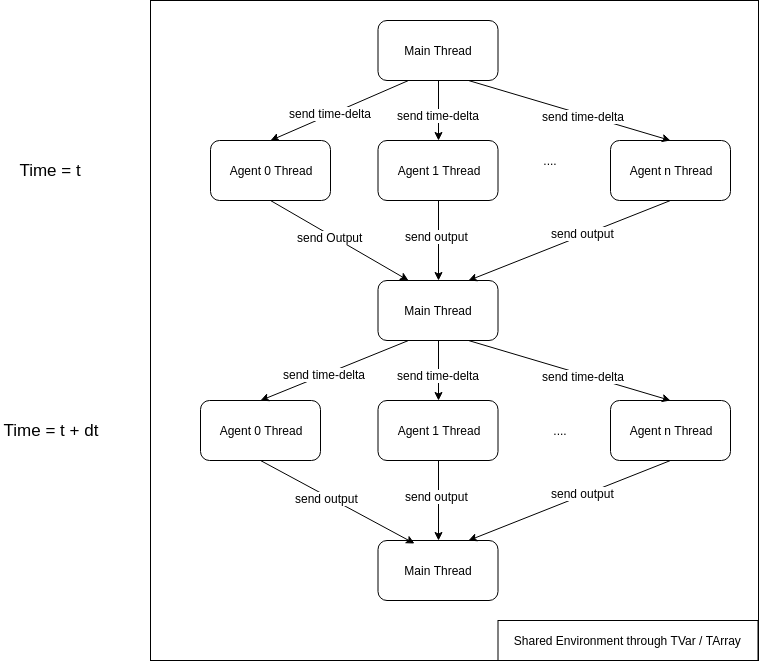
\includegraphics[width=0.7\textwidth, angle=0]{./fig/concurrentabs/stm_abs.png}
	\caption[Diagram of the parallel time-driven lock-step approach]{Diagram of the parallel time-driven lock-step approach.}
	\label{fig:stm_abs_structure}
\end{figure}

\subsection{Adding STM to agents}
We briefly discuss how to add STM to agents on a technical level and also show how to run them within their own threads. We use the SIR implementation as example - applying it to the Sugarscape implementation works exactly the same way and is left as a trivial exercise to the reader.

The first step is to simply add the \texttt{STM} Monad as the innermost level to the already the existing Transformer stack. Further, the environment is now passed as a transactional data primitive to the agent at \textit{construction time}. Thus, the agent does not receive the \texttt{SIREnv} as input any more but receives it through currying when constructing its initial \texttt{MSF}. Further, the agent modifies the \texttt{SIREnv} directly through the \texttt{TVar}, as demonstrated in the case of the infected agent.

\begin{HaskellCode}
-- Make Rand a transformer to be able to add STM as innermost monad
type SIRMonad g = RandT g STM
-- Input to agent is now an empty tuple instead of the Environment
type SIRAgent g = SF (SIRMonad g) () SIRState

-- The MSF construction function takes now the TVar with the environment.
sirAgent :: RandomGen g => TVar SIREnv -> Disc2dCoord -> SIRState -> SIRAgent g

-- The infected agent behaviour is nearly the same except that
-- the agent modifies the environment through the TVar
infected :: RandomGen g => SF (SIRMonad g) () (SIRState, Event ())
infected = proc _ -> do
  recovered <- occasionally illnessDuration () -< ()
  if isEvent recovered
    then (do
      -- update the environment through the TVar
      arrM_ (lift $ lift $ modifyTVar env (changeCell coord Recovered)) -< ()
      returnA -< (Recovered, Event ()))
    else returnA -< (Infected, NoEvent)
\end{HaskellCode}

The agent thread is straightforward. It takes \texttt{MVar} synchronisation primitives to synchronise with the main thread and simply runs the agent behaviour each time it receives the next \textit{DTime}:

\begin{HaskellCode}
agentThread :: RandomGen g 
            => Int             -- ^ Number of steps to compute
            -> SIRAgent g      -- ^ Agent behaviour MSF
            -> g               -- ^ Random-number generator of the agent
            -> MVar SIRState   -- ^ Synchronisation back to main thread
            -> MVar DTime      -- ^ Receiving DTime for next step
            -> IO ()
agentThread 0 _ _ _ _ = return () -- all steps computed, terminate thread
agentThread n sf rng retVar dtVar = do
  -- wait for dt to compute current step
  dt <- takeMVar dtVar

  -- compute output of current step
  let sfReader = unMSF sf ()
      sfRand   = runReaderT sfReader dt
      sfSTM    = runRandT sfRand rng
  -- run the STM action atomically within IO
  ((ret, sf'), rng') <- atomically sfSTM 

  -- post result to main thread
  putMVar retVar ret
  
  -- tail recursion to next step 
  agentThread (n - 1) sf' rng' retVar dtVar
\end{HaskellCode}

Computing a simulation step is now trivial within the main thread. All agent threads \texttt{MVars} are signalled to unblock followed by an immediate block on the \texttt{MVars} into which the agent threads post back their result. The state of the current step is then extracted from the environment, which is stored within the \texttt{TVar} which the agent threads have updated.

\begin{HaskellCode}
simulationStep :: TVar SIREnv     -- ^ environment 
               -> [MVar DTime]    -- ^ sync dt to threads
               -> [MVar SIRState] -- ^ sync output from threads
               -> DTime           -- ^ time delta
               -> IO SIREnv
simulationStep env dtVars retVars dt = do
  -- tell all threads to continue with the corresponding DTime
  mapM_ (`putMVar` dt) dtVars
  -- wait for results but ignore them, SIREnv contains all states
  mapM_ takeMVar retVars
  -- return state of environment when step has finished
  readTVarIO env
\end{HaskellCode}

The difference to an implementation which uses \texttt{IO} are minor but far reaching. Instead of using \texttt{STM} as innermost Monad, we use \texttt{IO}, thus running the whole agent behaviour within the \texttt{IO} Monad. Instead of receiving the environment through a \texttt{TVar}, the agent receives it through an \texttt{IORef}. It also receives an \texttt{MVar} which is the synchronisation primitive to synchronise the access to the environment in the \texttt{IORef} amongst all agents. Agents grab and release the synchronisation lock of the \texttt{MVar} when they enter and leave a critical section in which they operate on the environment stored in the \texttt{IORef}.

\section{Case Study I: SIR}
\label{sec:concurrent_sir}
Our first case study is the SIR model as introduced in Chapter \ref{sec:sir_model}. The aim of this case study is to investigate the potential speed up a concurrent \textit{STM} implementation gains over a sequential one under varying number of CPU cores and agents. The behaviour of the agents is quite simple and the interactions are happening indirectly through the environment, where reads from the environment outnumber the writes to it by far. Further, a comparison to a lock-based implementation with the \textit{IO} Monad is done to understand that \textit{STM} is also able to outperform traditional concurrency, \textit{in a pure functional ABS setting} while still retaining its greater static guarantees than \textit{IO} \footnote{The code of all three implementations is available at \url{https://github.com/thalerjonathan/phd/tree/master/public/stmabs/code/SIR}}.

\begin{enumerate}
	\item Sequential - this is the original implementation as discussed in Chapter \ref{sec:adding_env}, where the discrete 2D environment is shared amongst all agents as read-only data and the agents are executed sequentially within the main thread without any concurrency.
	\item STM - this is the same implementation as the \textit{Sequential} one but agents run now in the \textit{STM} Monad and have access to the discrete 2D environment through a transactional variable \textit{TVar}. This means that the agents now communicate indirectly by reads and writes through the \textit{TVar}.
	\item Lock-Based - this follows the \textit{STM} implementation, with the agents running in \textit{IO}. They share the discrete 2D environment using an \textit{IORef} and have access to an \textit{MVar} lock to synchronise access to it.
\end{enumerate}

Each experiment was run until $t = 100$ and stepped using $\Delta t = 0.1$. For each experiment we conducted 8 runs on our machine (see Table \ref{tab:machine_specs}) under no additional work-load and report the mean. %Further, we checked the visual outputs and the dynamics and they look qualitatively the same as the reference \textit{Sequential}. We could have used more rigour and properly validated the implementations against the formal specification using tests as we do in Chapter Property-based testing but we leave this for further res.
In the experiments we varied the number of agents (grid size) as well as the number of cores when running concurrently - the numbers are always indicated clearly.

\begin{table}
	\centering
	\begin{tabular}{ c || c }
		OS & Fedora 28, 64-bit \\ \hline
		RAM & 16 GByte \\ \hline
		CPU & Intel i5-4670K @ 3.4GHz \\ \hline
		HD & 250Gbyte SSD \\ \hline
		Haskell & GHC 8.2.2
	\end{tabular}
	
	\caption{Machine and Software specs for all experiments}
	\label{tab:machine_specs}
\end{table}

\subsection{Constant Grid Size, Varying Cores}
In this experiment we held the grid size constant to 51 x 51 (2,601 agents) and varied the cores. The results are reported in Table \ref{tab:constgrid_varyingcores}.

\begin{table}
	\centering
	\begin{tabular}{cc|c}
		\multicolumn{1}{ c||  }{\multirow{2}{*}{} } &
		\multicolumn{1}{ |c| }{Cores} & Duration      \\ \hline \hline 
		
		\multicolumn{1}{ c||  }{\multirow{1}{*}{Sequential} } &
		\multicolumn{1}{ |c| }{1} & 72.5      \\ \hline \hline 
		
		\multicolumn{1}{ c||  }{\multirow{4}{*}{Lock-Based} } &
		\multicolumn{1}{ |c| }{1} & 60.6       \\ \cline{2-3}
		\multicolumn{1}{ c||  }{}                       &
		\multicolumn{1}{ |c| }{2} & 42.8    \\ \cline{2-3}
		\multicolumn{1}{ c||  }{}                       &
		\multicolumn{1}{ |c| }{3} & 38.6    \\ \cline{2-3}
		\multicolumn{1}{ c||  }{}                       &
		\multicolumn{1}{ |c| }{4} & 41.6    \\ \hline \hline 
		
		\multicolumn{1}{ c||  }{\multirow{4}{*}{STM} } &
		\multicolumn{1}{ |c| }{1} & 53.2       \\ \cline{2-3}
		\multicolumn{1}{ c||  }{}                       &
		\multicolumn{1}{ |c| }{2} & 27.8    \\ \cline{2-3}
		\multicolumn{1}{ c||  }{}                       &
		\multicolumn{1}{ |c| }{3} & 21.8    \\ \cline{2-3}
		\multicolumn{1}{ c||  }{}                       &
		\multicolumn{1}{ |c| }{4} & \textbf{20.8}    \\ \hline \hline 
	\end{tabular}
  	
  	\caption{Experiments on 51x51 (2,601 agents) grid with varying number of cores. Timings in seconds (lower is better).}
	\label{tab:constgrid_varyingcores}
\end{table}

The \textit{STM} implementation running on 4 cores shows a speed up factor of 3.6 over \textit{Sequential}, which is a quite impressive number when considering that we can achieve at most a factor of 4 when running on 4 cores. It seems that \textit{STM} allow us to push the practical limit very close to the theoretical one, whereas the \textit{Lock-Based} approach just arrives at a factor of 1.74 on 4 cores.

Comparing the performance and scaling to multiple cores shows that the \textit{STM} implementation significantly outperforms the \textit{Lock-Based} one and scales better to multiple cores. The \textit{Lock-Based} implementation performs best with 3 cores and shows slightly worse performance on 4 cores as can be seen in Figure \ref{fig:core_duration_stm_io}. This is no surprise because the more cores are running at the same time, the more contention for the lock, thus the more likely synchronisation happening, resulting in higher potential for reduced performance. This is not an issue in \textit{STM} because no locks are taken in advance. 

\begin{figure}
	\centering
	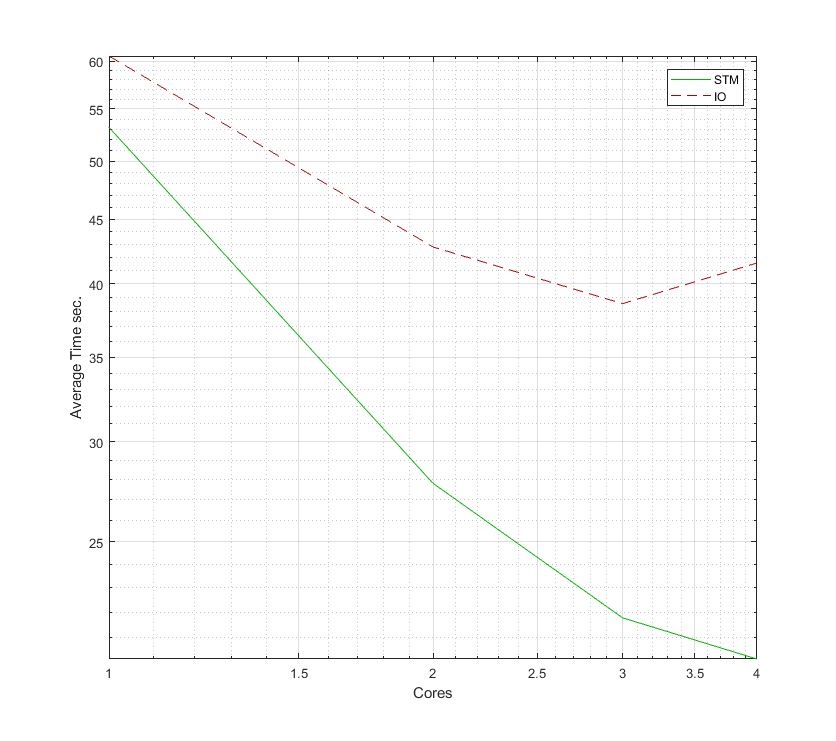
\includegraphics[width=0.8\textwidth, angle=0]{./fig/concurrentabs/sir/core_duration_stm_io.png}
	\caption{Comparison of performance and scaling on multiple cores of STM and Lock-Based. Note that the Lock-Based implementation seems to perform slightly worse on 4 than on 3 cores probably due to lock-contention.}
	\label{fig:core_duration_stm_io}
\end{figure}

\subsection{Varying Grid Size, Constant Cores}
In this experiment we varied the grid size and used always 4 cores. The results are reported in Table \ref{tab:varyinggrid_constcores} and plotted in Figure \ref{fig:varyinggrid_constcores}.

\begin{table}
	\centering
  	\begin{tabular}{ c || c | c | c }
        Grid-Size          & STM              & Lock-Based   & Ratio \\ \hline \hline 
   		51 x 51 (2,601)    & \textbf{20.2}    & 41.9         & 2.1 \\ \hline
   		101 x 101 (10,201) & \textbf{74.5}    & 170.5        & 2.3 \\ \hline
   		151 x 151 (22,801) & \textbf{168.5}   & 376.9        & 2.2 \\ \hline
   		201 x 201 (40,401) & \textbf{302.4}   & 672.0        & 2.2 \\ \hline
   		251 x 251 (63,001) & \textbf{495.7}   & 1,027.3      & 2.1 \\ \hline \hline
  	\end{tabular}

  	\caption{Performance on varying grid sizes. Timings in seconds (lower is better). Ratio compares STM to Lock-Based.}
	\label{tab:varyinggrid_constcores}
\end{table}

It is clear that the \textit{STM} implementation outperforms the \textit{Lock-Based} implementation by a substantial factor.

\begin{figure}
	\centering
	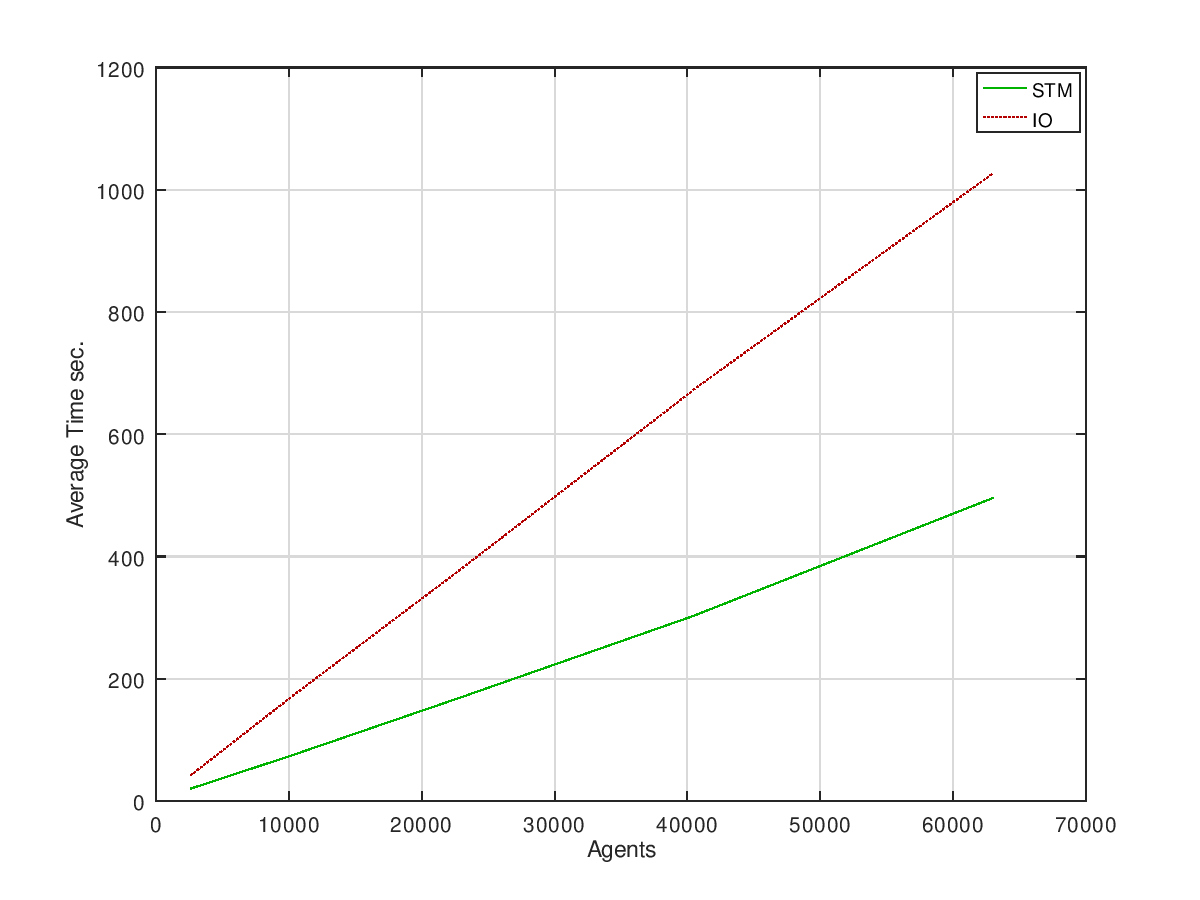
\includegraphics[width=1\textwidth, angle=0]{./fig/concurrentabs/sir/stm_io_varyinggrid_performance.png}
	\caption{Performance on varying grid sizes.}
	\label{fig:varyinggrid_constcores}
\end{figure}

\subsection{Retries}
Of very much interest when using STM is the retry-ratio, which obviously depends highly on the read-write patterns of the respective model. We used the \textit{stm-stats} library to record statistics of commits, retries and the ratio. The results are reported in Table \ref{tab:retries_stm}.

\begin{table}
	\centering
  	\begin{tabular}{ c || c | c | c }
        Grid-Size 		   & Commits    & Retries & Ratio \\ \hline \hline 
   		51 x 51 (2,601)    & 2,601,000  & 1306.5  & 0.0 \\ \hline
   		101 x 101 (10,201) & 10,201,000 & 3712.5  & 0.0 \\ \hline
   		151 x 151 (22,801) & 22,801,000 & 8189.5  & 0.0 \\ \hline
   		201 x 201 (40,401) & 40,401,000 & 13285.0 & 0.0 \\ \hline 
   		251 x 251 (63,001) & 63,001,000 & 21217.0 & 0.0 \\ \hline \hline
  	\end{tabular}
  	
  	\caption{Retry ratios on varying grid sizes on 4 cores.}
	\label{tab:retries_stm}
\end{table}

Independent of the number of agents we always have a retry-ratio of 0.0. This indicates that this model is \textit{very} well suited to STM, which is also directly reflected in the much better performance over the \textit{Lock-Based} implementation. Obviously this ratio stems from the fact that in our implementation we have \textit{very} few writes, which happen only in case when an agent changes from Susceptible to Infected or from Infected to Recovered. On the other hand, there are a very large number of reads due to indirect agent interaction. For \textit{STM} this is no problem because no lock is taken but the \textit{Lock-Based} approach is forced to conservatively take the lock to ensure mutual exclusive access to the critical section across all agents.

\subsection{Going Large-Scale}
To test how far we can scale up the number of cores in both the \textit{Lock-Based} and \textit{STM} cases, we ran two experiments, 51x51 and 251x251, on Amazon EC2 instances with a larger number of cores than our local machinery, starting with 16 and 32 to see if we are running into decreasing returns. The results are reported in Table \ref{tab:sir_varying_cores_amazon}.

\begin{table}
	\centering
  	\begin{tabular}{cc|c|c}
		\multicolumn{1}{ c||  }{\multirow{2}{*}{} } &
		\multicolumn{1}{ |c| }{Cores} & 51x51    & 251x251       \\ \hline \hline 
		
		\multicolumn{1}{ c||  }{\multirow{2}{*}{Lock-Based} } &
		\multicolumn{1}{ |c| }{16} & 72.5    & 1830.5       \\ \cline{2-4}
		\multicolumn{1}{ c||  }{}                       &
		\multicolumn{1}{ |c| }{32} & 73.1    & 1882.2      \\ \hline \hline 
		
		\multicolumn{1}{ c||  }{\multirow{2}{*}{STM} } &
		\multicolumn{1}{ |c| }{16} & \textbf{8.6}     & \textbf{237.0}       \\ \cline{2-4}
		\multicolumn{1}{ c||  }{}                       &
		\multicolumn{1}{ |c| }{32} & 12.0    & 248.7      \\ \hline \hline 
	\end{tabular}

  	\caption{Performance on varying cores on Amazon S2 Services. Timings in seconds (lower is better).}
	\label{tab:sir_varying_cores_amazon}
\end{table}

As expected, the \textit{Lock-Based} approach doesn't scale up to many cores because each additional core brings more contention to the lock, resulting in an even more decreased performance, even worse than the \textit{Sequential} implementation. This is particularly obvious in the 251x251 experiment because of the much larger number of concurrent agents. The \textit{STM} approach returns better performance on 16 cores but fails to scale further up to 32 where the performance drops below the one with 16 cores. In both STM cases we measured a retry-ratio of 0, thus we assume that with 32 cores we become limited by the overhead of STM transactions \cite{perfumo_limits_2008} because the workload of an STM action in our SIR implementation is quite small.

Compared to the \textit{Sequential} implementation, \textit{STM} reaches a speed up factor of 8.4 on 16 cores, which is still impressive but is much further away from the theoretical limit than in the case of only 4 cores -  a further indication that this model in particular and our approach in general does not scale up arbitrarily.

% NOTE: 0 retries in both cases means that the STM transactions themselves are becoming the bottleneck. this makes sens because the STM trasnactions in our SIR implementation are very small (especially recovered and infected agent) and could therefore really cause substantial overhead as pointed out by \cite{perfumo_limits_2008}
%16 cores 251x251: 0.0 retry-ratio
%32 cores 251x251: 0.0 retry ratio
%
%16 cores 51x51: 0.0 retry-ratio
%32 cores 51x51: 0.0 retry ratio

\subsection{Discussion}
The timing measurements speak a clear language: running in \textit{STM} and sharing state using a transactional variable \textit{TVar} is much more time-efficient than both the \textit{Sequential} and \textit{Lock-Based} approach. On 4 cores \textit{STM} achieves a speed up factor of 3.6, nearly reaching the theoretical limit.
Obviously both \textit{STM} and \textit{Lock-Based} sacrifices determinism: repeated runs might not lead to same dynamics despite same initial conditions. Still, by sticking to \textit{STM}, we get the guarantee that the source of this non-determinism is concurrency within the \textit{STM} monad but \textit{nothing else}. This we can not guarantee in the case of the \textit{Lock-Based} approach as all bets are off when running within \textit{IO}. The fact to have \textit{both} the better performance \textit{and} the stronger static guarantees in the \textit{STM} approach makes it \textit{very} compelling.

\section{Case Study II: Sugarscape}
\label{sec:sugarscape_concurrent}
The second case study is the Sugarscape model as introduced in Chapter \ref{sec:sugarscape}. In this case study we look into the potential performance improvement in a model with much more complex agent behaviour and dramatically increased writes on the shared environment.

We implemented the \textit{Carrying Capacity} (p. 30) section of Chapter II of the Sugarscape book \cite{epstein_growing_1996}. In each step agents search (move) to the cell with the most sugar they see within their vision, harvest all of it from the environment and consume sugar because of their metabolism. Sugar regrows in the environment over time. Only one agent can occupy a cell at a time. Agents don't age and cannot die from age. If agents run out of sugar due to their metabolism, they die from starvation and are removed from the simulation. The authors report that the initial number of agents quickly drops and stabilises around a level depending on the model parameters. This is in accordance with our results as we show in Chapter \ref{ch:property} and guarantees that we don't run out of agents. The model parameters are as follows:

\begin{itemize}
	\item Sugar Endowment: each agent has an initial sugar endowment randomly uniform distributed between 5 and 25 units;
	\item Sugar Metabolism: each agent has a sugar metabolism randomly uniform distributed between 1 and 5;
	\item Agent Vision: each agent has a vision randomly uniform distributed between 1 and 6, same for each of the 4 directions (N, W, S, E);
	\item Sugar Growback: sugar grows back by 1.0 unit per step until the maximum capacity of a cell is reached;
	\item Agent Number: initially 500 agents;
	\item Environment Size: 50 x 50 cells with toroid boundaries which wrap around in both x and y dimension.
\end{itemize}

Note that in this implementation (as in the full Chapter II of the book), no direct and no synchronous agent-interactions as we implemented them in Chapter \ref{sec:eventdriven_implementation} are happening. As in the SIR example, all agents interact with each other indirectly through the shared environment. This allows us to regard the implementation as a time-driven, parallel one wherein each step agents act conceptually at the same time.

We compare four different implementations \footnote{The code is freely available at \url{https://github.com/thalerjonathan/phd/tree/master/public/stmabs/code/SugarScape}}:

\begin{enumerate}
	\item Sequential - All agents are run after another (including the environment) and the environment is shared amongst the agents using a \textit{StateT} transformer.
	\item Lock-Based - All agents are run concurrently in the \textit{IO} monad and the environment is shared between the agents, using an \textit{IORef} with the access synchronised through an \textit{MVar} lock.
	\item STM TVar - All agents are run concurrently in the \textit{STM} monad and the environment is shared using a \textit{TVar} between the agents.
	\item STM TArray - All agents are run concurrently in the \textit{STM} monad and the environment is shared using a \textit{TArray} between the agents. 
\end{enumerate}

We follow \cite{lysenko_framework_2008} and measure the average number of steps per second of the simulation over 60 seconds. For each experiment we conducted 8 runs on our machine (see Table \ref{tab:machine_specs}) under no additional work-load and report the average. In the experiments we varied the number of cores when running concurrently - the numbers are always indicated clearly.

%\paragraph{Output} Note that we omit the graphical rendering in the functional approach because it is a serious bottleneck taking up substantial amount of the simulation time. Although visual output is often important in ABS, it is not what we are interested here thus we completely omit it and only output the number of agents in the simulation at each step piped into a file, thus omitting slow output to the console \footnote{Note that we need to produce \textit{some} output because of Haskells laziness - if we wouldn't output anything from the simulation then the expressions would actually never be fully evaluated thus resulting in high number of steps per second but which obviously don't really reflect the true computations done.}.

\paragraph{Ordering} The model specification requires to shuffle agents before every step (Footnote 12 on page 26 \cite{epstein_growing_1996}). In the \textit{Sequential} approach we do this explicitly but in the \textit{Lock-Based} and both \textit{STM} approaches we assume this to happen automatically due to race-conditions in concurrency, thus we arrive at an effectively shuffled processing of agents: we implicitly assume that the order of the agents is \textit{effectively} random in every step. The important difference between the two approaches is that in the \textit{Sequential} approach we have full control over this randomness but in the \textit{STM} not - also this means that repeated runs with the same initial conditions might lead to slightly different results. 
This decision leaves the execution order of the agents ultimately to Haskell's Runtime System and the underlying OS. We are aware that by doing this, we make assumptions that the threads run uniformly distributed (fair) but such assumptions should not be made in concurrent programming. As a result we can expect this fact to produces non-uniform distributions of agent runs but we assumed that for this model this does not has a significance influence - in case of doubt, we could resort to shuffling the agents before running them in every step. We agree that this very problem would deserve in-depth research on its own, where also the influence of non-deterministic ordering on the correctness and results of ABS has to be analysed. This is not the main interest of this section though and we leave it for further research as it is completely beyond the focus of this thesis.

%Note that in the concurrent implementations we have two options for running the environment: either asynchronously as a concurrent agent at the same time with the population agents or synchronously after all agents have run. We must be careful though as running the environment as a concurrent agent can be seen as conceptually wrong because the time when the regrowth of the sugar happens is now completely random. In this case it could happen that sugar regrows in the very first transaction or in the very last, different in each step, which can be seen as a violation of the model specifications. Thus we do not run the environment concurrently with the agents but synchronously after all agents have run.

\subsection{Constant Agent Size}
In a first approach we compare the performance of all implementations on varying numbers of cores. The results are reported in Table \ref{tab:varying_cores} and plotted in Figure \ref{fig:varying_cores}. 

\begin{table}
	\centering
	\begin{tabular}{cc|c|c}
		\multicolumn{1}{ c||  }{\multirow{2}{*}{} } &
		\multicolumn{1}{ |c| }{Cores} & Steps & Retries      \\ \hline \hline 
		
		\multicolumn{1}{ c||  }{\multirow{1}{*}{Sequential} } &
		\multicolumn{1}{ |c| }{1} & 39.4 & N/A     \\ \hline \hline 
		
		\multicolumn{1}{ c||  }{\multirow{4}{*}{Lock-Based} } &
		\multicolumn{1}{ |c| }{1} & 43.0 & N/A       \\ \cline{2-4}
		\multicolumn{1}{ c||  }{}                       &
		\multicolumn{1}{ |c| }{2} & 51.8 & N/A   \\ \cline{2-4}
		\multicolumn{1}{ c||  }{}                       &
		\multicolumn{1}{ |c| }{3} & 57.4 & N/A   \\ \cline{2-4}
		\multicolumn{1}{ c||  }{}                       &
		\multicolumn{1}{ |c| }{4} & 58.1 & N/A   \\ \hline \hline 
		
		\multicolumn{1}{ c||  }{\multirow{4}{*}{STM \textit{TVar}} } &
		\multicolumn{1}{ |c| }{1} & \textbf{47.3} & 0.0       \\ \cline{2-4}
		\multicolumn{1}{ c||  }{}                       &
		\multicolumn{1}{ |c| }{2} & 53.5 & 1.1    \\ \cline{2-4}
		\multicolumn{1}{ c||  }{}                       &
		\multicolumn{1}{ |c| }{3} & 57.1 & 2.2    \\ \cline{2-4}
		\multicolumn{1}{ c||  }{}                       &
		\multicolumn{1}{ |c| }{4} & 53.0 & 3.2   \\ \hline \hline 
		
		\multicolumn{1}{ c||  }{\multirow{4}{*}{STM \textit{TArray}} } &
		\multicolumn{1}{ |c| }{1} & 45.4 & 0.0       \\ \cline{2-4}
		\multicolumn{1}{ c||  }{}                       &
		\multicolumn{1}{ |c| }{2} & \textbf{65.3} & 0.02   \\ \cline{2-4}
		\multicolumn{1}{ c||  }{}                       &
		\multicolumn{1}{ |c| }{3} & \textbf{75.7} & 0.04    \\ \cline{2-4}
		\multicolumn{1}{ c||  }{}                       &
		\multicolumn{1}{ |c| }{4} & \textbf{84.4} & 0.05   \\ \hline \hline 
	\end{tabular}  	
  	
  	\caption{Steps per second and retries on 50x50 grid with 500 initial agents on varying cores.}
	\label{tab:varying_cores}
\end{table}

\begin{figure}
	\centering
	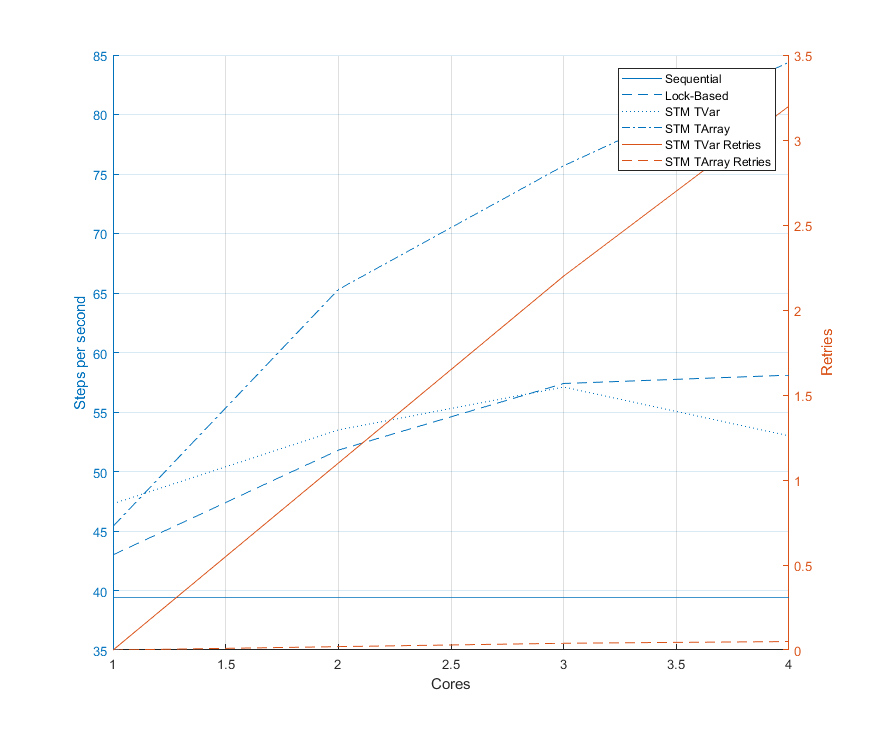
\includegraphics[width=0.7\textwidth, angle=0]{./fig/concurrentabs/sugarscape/varying_cores.png}
	\caption{Steps per second and retries on 50x50 grid and 500 initial agents on varying cores.}
	\label{fig:varying_cores}
\end{figure}

As expected, the \textit{Sequential} implementation is the slowest, followed by the \textit{Lock-Based} and \textit{TVar} approach whereas \textit{TArray} is the best performing one.

We clearly see that using a \textit{TVar} to share the environment is a very inefficient choice in this model: \textit{every} write to a cell leads to a retry independent whether the reading agent reads that changed cell or not, because the data-structure can not distinguish between individual cells. By using a \textit{TArray} we can avoid the situation where a write to a cell in a far distant location of the environment will lead to a retry of an agent which never even touched that cell. Also the \textit{TArray} seems to scale up by 10 steps per second for every core added. It will be interesting to see how far this could go with the Amazon experiment, as we seem not to hit a limit with 4 cores yet.

The inefficiency of \textit{TVar} is also reflected in the nearly similar performance of the \textit{Lock-Based} implementation which even outperforms it on 4 cores. This is due to very similar approaches because both operate on the whole environment instead of only the cells as \textit{TArray} does. This seems to be a bottleneck in \textit{TVar} reaching the best performance on 3 cores, which then drops on 4 cores due to an increasing retries ratio. The \textit{Lock-Based} approach seems to reduce its returns on increased number of cores hitting a limit at 4 cores as well.

\subsection{Scaling up Agents}
So far we kept the initial number of agents at 500, which due to the model specification, quickly drops and stabilises around 200 due to the carrying capacity of the environment as described in the book \cite{epstein_growing_1996} section \textit{Carrying Capacity} (p. 30).

We now want to measure the performance of our approaches under increased number of agents. For this we slightly change the implementation: always when an agent dies it spawns a new one which is inspired by the ageing and birthing feature of Chapter III in the book \cite{epstein_growing_1996}. This ensures that we keep the number of agents roughly constant (still fluctuates but doesn't drop to low levels) over the whole duration. This ensures a constant load of concurrent agents interacting with each other and demonstrates also the ability to terminate and create concurrent agents (threads) dynamically during the simulation.

Except for the \textit{Sequential} approach we ran all experiments with 4 cores (TVar with 3 as well). We looked into the performance of 500, 1,000, 1,500, 2,000 and 2,500 (maximum possible capacity of the 50x50 environment). The results are reported in Table \ref{tab:state_results_agentsscale_time} and plotted in Figure \ref{fig:state_results_agentsscale_time}.

\begin{table}
	\centering
  	\begin{tabular}{ c || c | c | c | c | c }
        Agents  & Sequential & Lock-Based & TVar (3 cores) & TVar (4 cores) & TArray  \\ \hline \hline 
    	    500     & 14.4       & 20.2		  &	20.1           & 18.5       	& \textbf{71.9}    \\ \hline
   		1,000   & 6.8        & 10.8 	      & 10.4           & 9.5         & \textbf{54.8}    \\ \hline
   		1,500   & 4.7        & 8.1 		  & 7.9            & 7.3			& \textbf{44.1}    \\ \hline
   		2,000   & 4.4        & 7.6 		  & 7.4            & 6.7    		& \textbf{37.0}    \\ \hline 
   		2,500   & 5.3        & 5.4 		  & 9.2            & 8.9			& \textbf{33.3}    \\ \hline \hline
   	\end{tabular}
  	
  	\caption{Steps per second on 50x50 grid with varying number of agents with 4 (and 3) cores except Sequential (1 core).}
	\label{tab:state_results_agentsscale_time}
\end{table}

\begin{figure}
	\centering
	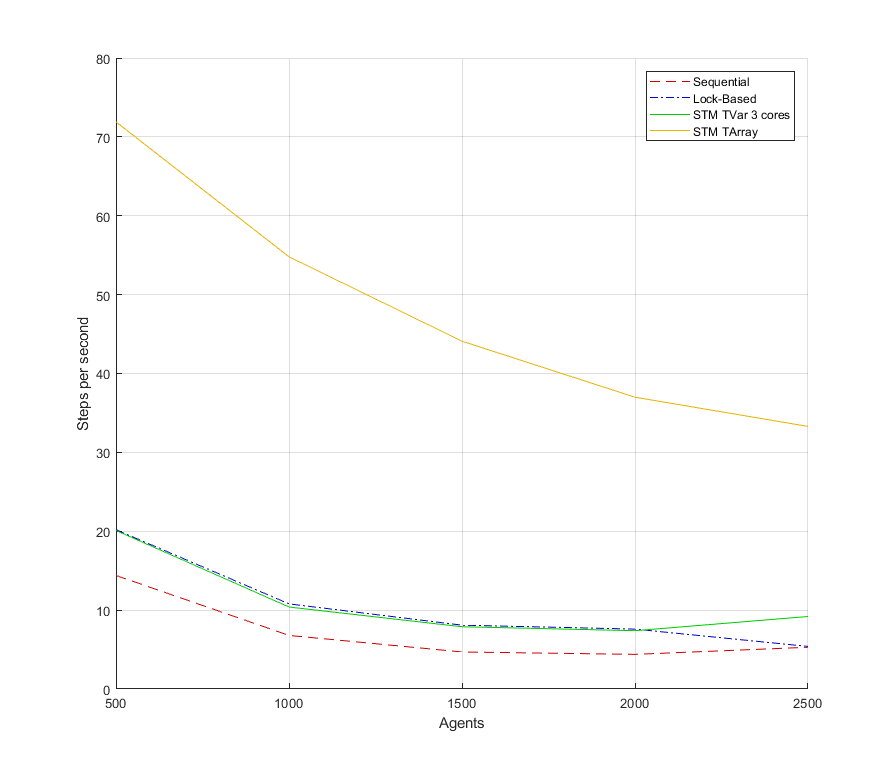
\includegraphics[width=1.0\textwidth, angle=0]{./fig/concurrentabs/sugarscape/varying_agents.png}
	\caption{Steps per second on 50x50 grid and varying number of agents with 4 (and 3) cores except Sequential (1 core).}
	\label{fig:state_results_agentsscale_time}
\end{figure}

As expected, the \textit{TArray} implementation outperforms all others substantially. Also as expected, the \textit{TVar} implementation on 3 cores is faster than on 4 cores as well when scaling up to more agents. The \textit{Lock-Based} approach performs about the same as the \textit{TVar} on 3 cores because of the very similar approaches: both access the \textit{whole} environment. Still the \textit{TVar} approach uses one core less to arrive at the same performance, thus strictly speaking outperforming the \textit{Lock-Based} implementation.

What seems to be very surprising is that in the \textit{Sequential} and \textit{TVar} cases the performance with 2,500 agents is \textit{better} than the one with 2,000 agents. The reason for this is that in the case of 2,500 agents, an agent can't move anywhere because all cells are already occupied. In this case the agent won't rank the cells in order of their pay-off (max sugar) to move to but just stays where it is. We hypothesize that due to Haskells laziness the agents actually never look at the content of the cells in this case but only the number which means that the cells themselves are never evaluated which further increases performance. This leads to the better performance in case of \textit{Sequential} and \textit{TVar} because both exploit laziness.
In the case of the \textit{Lock-Based} approach we still arrive at a lower performance because the limiting factor are the unconditional locks. In the case of the \textit{TArray} approach we also arrive at a lower performance because it seems that STM perform reads on the neighbouring cells which are not subject to lazy evaluation. In Haskell it is notoriously difficult to reason about efficiency (see Chapter \ref{ch:drawbacks} for a short discussion on drawbacks) and this behaviour of improved performance due to Haskells lazyness is no exception. We leave an in-depth investigation for further research as it is beyond the focus of this chapter.

We also measured the average retries both for \textit{TVar} and \textit{TArray} under 2,500 agents where the \textit{TArray} approach shows best scaling performance with 0.01 retries whereas \textit{TVar} averages at 3.28 retries. Again this can be attributed to the better transactional data-structure which reduces retry-ratio substantially to near-zero levels.

\subsection{Going Large-Scale}
To test how far we can scale up the number of cores in both the \textit{Lock-Based} and \textit{TArray} cases, we ran the two experiments (carrying capacity and rebirthing) on Amazon EC2 instances with increasing number of cores starting with 16 and 32 to see if we run into decreasing returns. The results are reported in Table \ref{tab:sug_varying_cores_amazon}.

\begin{table}
	\centering
%  	\begin{tabular}{ c || c | c | c }
%                   & Cores & Carrying Capacity & Rebirthing  \\ \hline \hline 
%    	Lock-Based & 16    & 53.9              & 4.4         \\ \hline
%    	Lock-Based & 32    & 44.2              & 3.6         \\ \hline \hline 
%   		
%   		STM TArray & 16    & \textbf{116.8} (0.23)      & \textbf{39.5} (0.08) \\ \hline
%   		STM TArray & 32    & 109.8 (0.41)      & 31.3 (0.18) \\ \hline \hline 
%   	\end{tabular}
  	
	\begin{tabular}{cc|c|c}
		\multicolumn{1}{ c||  }{\multirow{2}{*}{} } &
		\multicolumn{1}{ |c| }{Cores} & Carrying Capacity    & Rebirthing       \\ \hline \hline 
		
		\multicolumn{1}{ c||  }{\multirow{2}{*}{Lock-Based} } &
		\multicolumn{1}{ |c| }{16} & 53.9              & 4.4       \\ \cline{2-4}
		\multicolumn{1}{ c||  }{}                       &
		\multicolumn{1}{ |c| }{32} & 44.2              & 3.6      \\ \hline \hline 
		
		\multicolumn{1}{ c||  }{\multirow{2}{*}{STM TArray} } &
		\multicolumn{1}{ |c| }{16} & \textbf{116.8} (0.23)      & \textbf{39.5} (0.08)       \\ \cline{2-4}
		\multicolumn{1}{ c||  }{}                       &
		\multicolumn{1}{ |c| }{32} & \textbf{109.8} (0.41)      & \textbf{31.3} (0.18)      \\ \hline \hline 
	\end{tabular}  	
  	
  	\caption{Steps per second on varying cores on Amazon S2 Services.}
	\label{tab:sug_varying_cores_amazon}
\end{table}

As expected, the \textit{Lock-Based} approach doesn't scale up to many cores because each additional core brings more contention to the lock, resulting in even more decreased performance. This is particularly obvious in the rebirthing experiment because of the much larger number of concurrent agents. The \textit{TArray} approach returns better performance on 16 cores but fails to scale further up to 32 where the performance drops below the one with 16 cores. We indicated the retry-ratio in brackets and see that they roughly double from 16 to 32, which is the reason why performance drops as at this point. 

%the INCREASE in time can only happen due to more retries
%Carrying Capacity 16 core ~ 0.23 retry-ratio
%Carrying Capacity 32 core ~ 0.41 retry-ratio
%
%Rebirthing 16 core ~ 0.08 retry-ratio
%Rebirthing 32 core ~ 0.18 retry-ratio

\subsection{Comparison with other approaches}
The paper \cite{lysenko_framework_2008} reports a performance of 17 steps in RePast, 18 steps in MASON (both non-parallel) and 2,000 steps per second on a GPU on a 128x128 grid. Although our \textit{Sequential} implementation, which runs non-parallel as well, outperforms the RePast and MASON implementations of \cite{lysenko_framework_2008}, one must be very well aware that these results were generated in 2008, on current hardware of that time.

%When we run the SugarScape example of RePast with the same model parameters as ours on the same machine (see Table \ref{tab:machine_specs}) we arrive at roughly 450 steps per second - a factor of about 3.8 faster than even our STM \textit{TArray} implementation on 16 cores. This might seem quite shocking, even more so because RePast also performs visual output, rendering the SugarScape in every step. When scaling up the agents to 2,500 the RePast version arrives around roughly 95 steps per second which is still faster by a factor of 3 than our 4 core \textit{TArray} implementation. We attribute this substantial performance difference to the inherent performance difference of functional programming to imperative approaches as already outlined in the previous section. 

The very high performance on the GPU does not concern us here as it follows a very different approach than ours. We focus on speeding up implementations on the CPU as directly as possible without locking overhead. When following a GPU approach one needs to map the model to the GPU which is a delicate and non-trivial matter. With our approach we show that speed up with concurrency is very possible without the low-level locking details or the need to map to GPU. Also some features as bilateral trading between agents, where a pair of agents needs to come to a conclusion over multiple synchronous steps, is difficult to implement on a GPU whereas this is easily possible using STM.

Note that we kept the grid-size constant because we implemented the environment as a single agent which works sequentially on the cells to regrow the sugar. Obviously this doesn't really scale up on parallel hardware and experiments which we haven't included here due to lack of space, show that the performance goes down dramatically when we increase the environment to 128x128 with same number of agents which is the result of Amdahl's law where the environment becomes the limiting factor of the simulation. Depending on the underlying data-structure used for the environment we have two options to solve this problem. In the case of the \textit{Sequential} and \textit{TVar} implementation we build on an indexed array, which we can be updated in parallel using the existing data-parallel support in Haskell. In the case of the \textit{TArray} approach we have no option but to run the update of every cell within its own thread. We leave both for further research as it is out of scope of this paper.

\subsection{Discussion}
This case study showed clearly that besides being substantially faster than the \textit{Sequential} implementation, \textit{STM} is also able to perform considerably better than a \textit{Lock-Based} approach even in the case of a model with much higher complexity in agent behaviour and dramatically increased number of writes to the environment.
Further, this case study demonstrated that the selection of the right transactional data-structure is of fundamental importance when using \textit{STM}. Selecting the right transactional data-structure is very model-specific and can lead to dramatically different performance results.
In this case the \textit{TArray} performed best due to many writes but in the SIR case-study a \textit{TVar} showed good enough results due to the very low number of writes. When not carefully selecting the right transactional data-structure which supports fine-grained concurrency, a lock-based implementation might perform as well or even outperform the STM approach as can be seen when using the \textit{TVar}.
Although the \textit{TArray} is the better transactional data-structure overall, it might come with an overhead, performing worse on low number of cores than a \textit{TVar} approach but has the benefit of quickly scaling up to multiple cores. Depending on the transactional data-structure, scaling up to multiple cores hits a limit at some point. In the case of the \textit{TVar} the best performance is reached with 3 cores. With the \textit{TArray} we reached this limit around 16 cores.

Note that the comparison between the \textit{Lock-Based} approach and the \textit{STM TArray} implementation is a bit unfair due to a very different locking structure. A more suitable comparison would have been to use an indexed Array with a tuple of (MVar, IORef) in each cell to support fine-grained locking on cell-level. This would be a more just comparison to the \textit{STM Array} where fine-grained transactions happen on the cell-level. We hypothesize that \textit{STM} will still outperform the \textit{IO} approach but to a lesser degree - we leave the proof of this for further research.

%Unfortunately, for this model the performance is nowhere comparable to imperative approaches, which we attribute to the inherent performance difference of functional programming to imperative approaches. With the use of advanced language features we might arrive at much improved performance but we leave this for further research as we focus primarily on the comparison between lock-based and STM approaches.

%we can implement everything except synchronous direct agent-interactions atm: if agent-interaction is one-way e.g. paying back a loan then this is no problem. thus the following parts of the Sugarscape are not possible with our current STM approach: mating, trading and lending  because all 3 require direct agent-to-agent interaction over multiple steps. We leave the problem of developing such an algorithm / implementation for further research.

\section{Discussion}
Although there are similarities to the work of \cite{botta_time_2010} (the use of messages and the problem of when to advance time in models with arbitrary number synchronised agent-interactions), we approach our agents differently. First in our approach an agent is only a single MSF and thus can not be directly queried for its internal state / its id or outgoing messages, instead of taking a list of messages, our agents take a single event/message and can produce an arbitrary number of outgoing messages together with an observable state - note that this would allow to query the agent for its id and its state as well by simply sending a corresponding message to the agents MSF and requiring the agent to implement message handling for it. Also the state of our agents is \textit{completely} localised and there is no means of accessing the state from outside the agent, they are thus "fully encapsulated agents" \cite{botta_time_2010}. Note that the authors of \cite{botta_time_2010} define their agents with a polymorphic agent-state type \textit{s}, which implies that without knowledge of the specific type of \textit{s} there would be no way of accessing the state, rendering it in fact also fully encapsulated. The problem of advancing time in our approach is solved not exactly the same but conceptually it is the same: after sending a tick message to each agent (in random order), we process all agents until they are idle: there are no more enqueued messages / events in the queue.

our eventdriven approach makes heavy use of 2 state monads, thus one might ask what the benefits are, after all we seem to fall back into stateful, imperative style programming. we agree that our approach is just one way of implementing abs in fp but we think we have come a long way thus making our approach quite valuable even if there might be other approaches like shallow EDSLs. on the other hand even our stateful programming is highly restricted to only those 2 local datatypes which makes it much more manageable than unrestricted data mutation

quote carmack (\url{http://www.gamasutra.com/view/news/169296/Indepth_Functional_programming_in_C.php}): the main difficulty as a developer in software programming is to keep track of the states a program can be in and reason about them and their Validity

TODO: report LoC and compare it with other implementations we found on the internet

\chapter{Verification \& Correctness}
Testing of functional ABS paper
10\%

- correctness \& verification
	-> static type system eliminates a large number run-time bugs: if we decide to rule out IO then we can guarantee 


\chapter{Dependent Types}
%My work is all nice and good but it solves problems the ABS community and implementations never really had. My FRP/MSF approach is quite complex and can be equally difficult to get right. Even worse, the bugs were not primarily those I am solving with FP but the REAL problem in ABS is translating the model into code. Can FP help us here? Can my pure FP approach help here? expressing invariants in FP code? can we express them in types? 

The pure functional implementation techniques have a number of technical benefits but don't help as much in closing the gap between specification and implementation as one is used from functional programming in general. Therefore we take a step back and abstract from these highly complex implementation techniques and move towards dependent types. Follow \cite{botta_time_2010} and \cite{botta_functional_2011}.

Conceptually discuss how dependent types can be made of use in ABS without going into lot of technical detail because: 1. i didn't do enough research on it and 2. dependent types seem to be nearly out of focus of the thesis.

%Linear and Dependent Types with Idris 2: more general ideas / hints / research on how it is applicable to ABS

%dependent types in ABS paper, explore totality - equilibrium correspondence idea
%About 20\% finished.

\section{Case-Study}
perform gintis case-study: apply my developed techniques of implementing ABS and testing and concurrency / parallelism to the gintis paper (and its follow ups: the ionescu paper and the masterthesis on it). 
The aim of this is to see: 

1. do the techniques transfer to this problem? 
2. does haskell prevent making that mistake which gintis made? 
3. how close is our implementation to ionescus functional specification? 
4. validation and verification against gintis paper using property-based testing of individual agents and the simulation as a whole. 
5. being more familiar with dependent types, would they help and where do they fit in in combination with the ionescu functional specification, which mentions dependent types at the end.

\section{Discussion}
Although there are similarities to the work of \cite{botta_time_2010} (the use of messages and the problem of when to advance time in models with arbitrary number synchronised agent-interactions), we approach our agents differently. First in our approach an agent is only a single MSF and thus can not be directly queried for its internal state / its id or outgoing messages, instead of taking a list of messages, our agents take a single event/message and can produce an arbitrary number of outgoing messages together with an observable state - note that this would allow to query the agent for its id and its state as well by simply sending a corresponding message to the agents MSF and requiring the agent to implement message handling for it. Also the state of our agents is \textit{completely} localised and there is no means of accessing the state from outside the agent, they are thus "fully encapsulated agents" \cite{botta_time_2010}. Note that the authors of \cite{botta_time_2010} define their agents with a polymorphic agent-state type \textit{s}, which implies that without knowledge of the specific type of \textit{s} there would be no way of accessing the state, rendering it in fact also fully encapsulated. The problem of advancing time in our approach is solved not exactly the same but conceptually it is the same: after sending a tick message to each agent (in random order), we process all agents until they are idle: there are no more enqueued messages / events in the queue.

our eventdriven approach makes heavy use of 2 state monads, thus one might ask what the benefits are, after all we seem to fall back into stateful, imperative style programming. we agree that our approach is just one way of implementing abs in fp but we think we have come a long way thus making our approach quite valuable even if there might be other approaches like shallow EDSLs. on the other hand even our stateful programming is highly restricted to only those 2 local datatypes which makes it much more manageable than unrestricted data mutation

quote carmack (\url{http://www.gamasutra.com/view/news/169296/Indepth_Functional_programming_in_C.php}): the main difficulty as a developer in software programming is to keep track of the states a program can be in and reason about them and their Validity

TODO: report LoC and compare it with other implementations we found on the internet

\chapter{Conclusions}
\label{chap:concl}

\section{Being Realistic}
It is of most importance to stress that we don't condemn the current state-of-the-art approach of object-oriented specification and implementation to ABS. The strength of object-oriented programming is surely that it can be seen as \textit{programming as modelling} and thus will be always an attractive approach to ABS. Also we are realists and know that there are more points to consider when selecting a set of methods for developing software for an ABS than robustness, verification and validation. Almost always the popularity of an existing language and which languages the implementer knows is the driving force behind which methods and languages to choose. This means that ABS will continue to be implemented in object-oriented programming languages and many perfectly well functioning models will be created by it in the future. Although they all suffer from the same issues mentioned in the introduction this doesn't matter as they are not of central importance to most of them.
Nonetheless we think our work is still essential and necessary as it may start a slow paradigm-shift and opens up the minds of the ABS community to a more functional and formal way of approaching and implementing agent-based models and simulations and recognizing the benefits one gets automatically from it by doing so.

\section{What we are not doing}
Because of this highly interdisciplinary topic we explicitly mention what we do not want to undertake in this PhD.
First we don't want to develop another language for formal agent-specification which needs to be compiled or used in some fancy tool - we want to put it directly into Haskell, building on the existing facilities.
Second, we are not developing a new economic theory about decentralized bilateral bartering, we take the existing theory and existing agent-based models and apply our methods to them.
Third, we don't want to use fancy statistics and number juggling for comparing validating and verifying models: we want structural comparison (category-theory).
Fourth, we do NOT want to do a direct comparison of object-orientation vs. functional in ABS, as we would get lost in an infinite amount of low-level technical details. We look at the benefits / drawbacks more on a conceptual level, applied to ABS.

\renewcommand\bibname{References}

\bibliographystyle{acm}
\bibliography{../../writing/references/phdReferences}

\begin{appendices}

\chapter{Pure Functional Epidemics}
\label{app:pfe}
Submission history:
\begin{enumerate}
	\item Submitted to Haskell Symposium 2018 on 30th March \\ REJECTED on 18th May
	\item Submitted to IFL 2018 on 25th May \\ NOTIFICATION PENDING until 20th July
\end{enumerate}

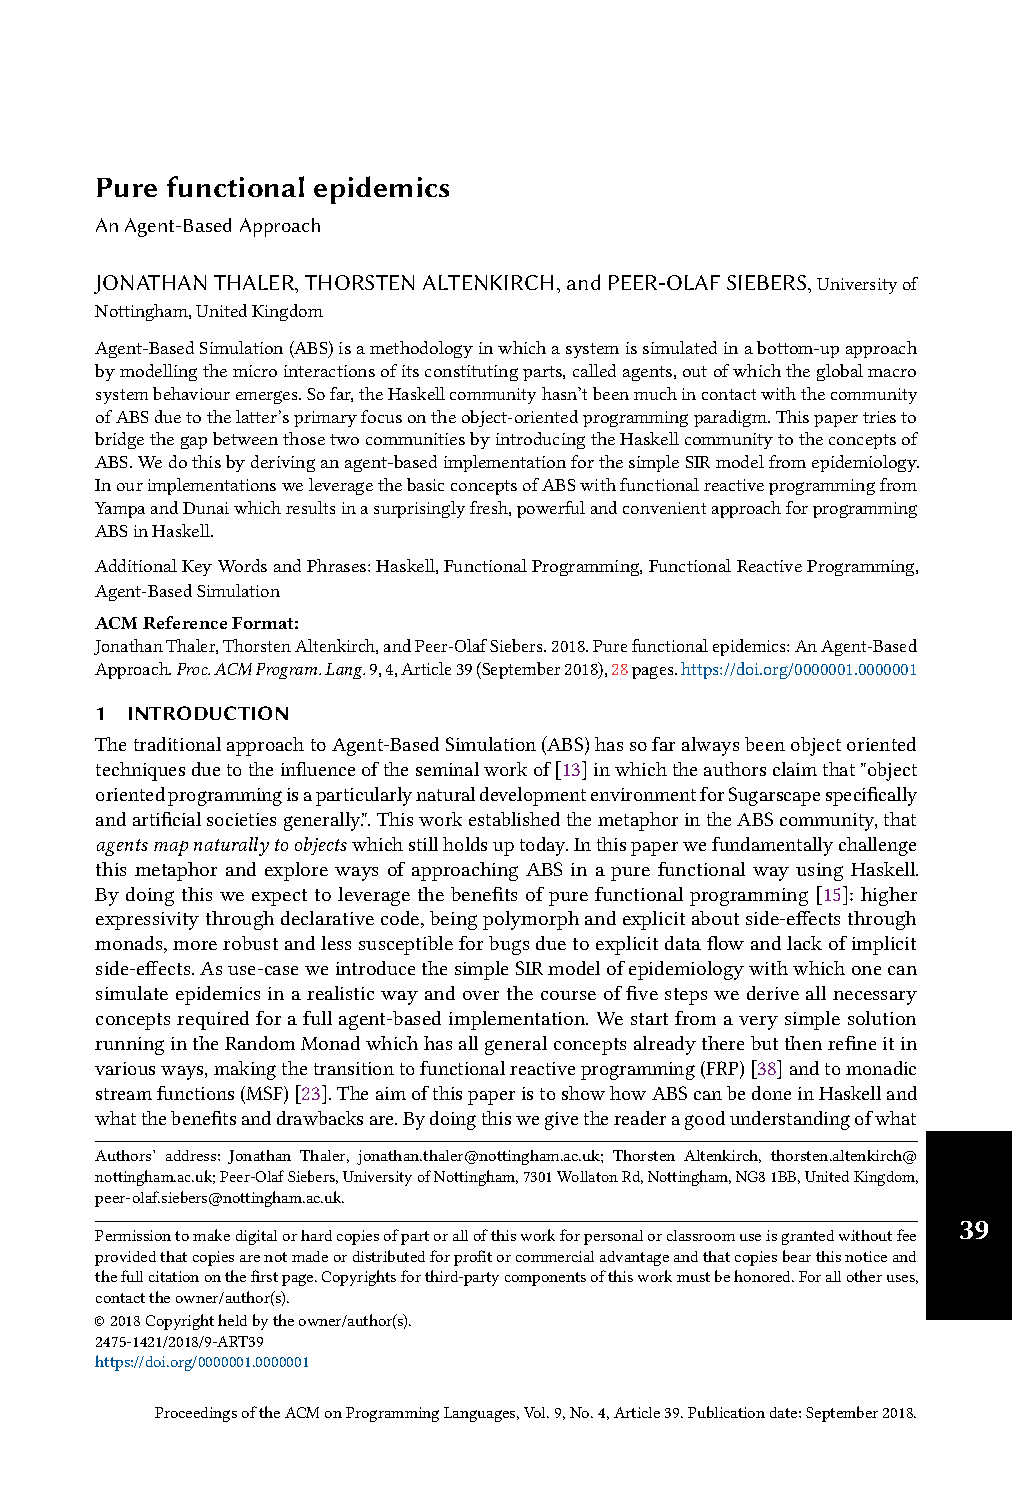
\includepdf[pages=-]{./pdf/pfe.pdf}

% NOTE: keep it out to the submission for the reviewers
%\chapter{Questions \& Answers}
\label{chap:qa}

TODO: update and adopt to 2nd year

In this chapter I give answers to anticipated questions and objections about my research direction and vision of doing pure functional ABS \footnote{They are not always posed in a dead-serious way but as it is a quite controversial topic - ABS should be done object-orientated after all huh? - I think it is appropriate. Also some objections were raised in exactly this way.}.

\paragraph{So you had this hypothesis, that pure functional programming and dependent types lead to simulation software which is more likely correct and is easier to verify and validate, right from the beginning?}
Not at all. I even had no deep knowledge of functional programming at the start of my PhD, I've just worked through the 1st edition of Grahams book "Programming in Haskell" and that's it. I had no clear understanding of purity, side-effects and Monads and I didn't know a bit about functional reactive programming. I knew that something like Dependent Types exist because Thorsten (2nd Supervisor) has sent me an email before the start of my PhD in which he pointed at Agda, so I started reading a bit about intuitionistic / constructivistic math, tried out a little bit of Agda but quickly gave up because it was way too far away (without really having mastered pure functional programming in Haskell, I believe it is nearly impossible / too difficult / makes no sense going into dependent types).
So in the beginning there was pure \textit{curiosity} about functional programming in combination with ABS because I knew nothing of FP at all and wanted to understand it (after getting bored by OO) and applying FP to ABS seemed so crazy (because everyone claims OO to be 'natural' for it) that it must be an extremely interesting challenge. I guess this is very often the case with research: there is 'just' curiosity in the beginning and then during the research process a hypothesis falls into place.


\chapter{Thesis Structure}
\label{app:thesis_struct}

TODO: find the story of my PhD thesis and connect it to my publication plan. 
TODO: story e.g. "We need functional programming to reduce the potential sources of bugs and introducing bugs harder, resulting in software which is more likely to be correct. Additionally by using dependent types we can narrow the gap between model specification and implementation even further, resulting in software which is even more likely to be correct. Further, additional benefits fall into place: purity leads to guaranteed reproducibility at compile-time, software transactional memory can be utilised to scale up to massively parallel and we have property-based testing at hand which puts the focus on specification testing rather than testing operational details".

This appendix gives a first draft of the structure outline of the thesis which I plan on start writing in April 2019. I aim for a flat structure which emphasises a strong narrative. The order of writing will be: Methodology, Proof-Of-Concept chapters, Literature Review, Discussion, Conclusions, Introduction, Abstract.
%
%line of argument
%1. established methods need extensive unit-testing for establishing correctness of software, which only increases the likelihood of correctness and doesnt guarantee it because they are inherent dynamic, testing run-time behaviour, because of the different type system.
%2. functional programming as in haskell has a strong static type system which allows to shift much much more guarantees towards static, compile-time, making many run-time tests obsolete and can guarantee a few things already at compile-time which makes tests to cover that completely obsolete
%3. dependent types can push these guarantees even further and theoretically should allow to express guarantees at compile-time to an arbitrary complex level which in theory should allow us to abandon run-time testing of bugs altogether. This does not mean that we don't need any tests anymore, as will be outlined in the chapter on Verification \& Validation \ref{chap:v_and_v}.
%4. with shifting more towards compile-time guarantees we automatically gain more confidence into the correctness of our simulation and reduce the implementation overhead of writing tests for those cases. Also some properties are simply not testable with run-time tests e.g. that some property holds forever - this is only possible to guarantee by looking at the code directly (where functional programming shines) or expressing it through compile-time guarantees. 
%5. correct by construction: narrowing the gap between model specification and implementation 
%6. Impedance Mismatch: ABS is constructive / generative in nature but the nature of the test-driven development process is deductive. is this a problem? Think of it more deeply


\section{Introduction}
This chapter is the introduction to the thesis and motivates it and describes the aim and scope of the Ph.D. Further it states the hypotheses and contributions.
\begin{itemize}
	\item Main Argument: Defining the problem, motivation, aim and scope of the Ph.D.
	\item Hypotheses: Precisely stating the hypotheses which will form the points of reference for the whole research.
	\item Contributions: Precisely list the contribution to knowledge this Ph.D. makes and list all papers which were written (and published) during this Ph.D.
\end{itemize}

\section{Literature Review}
This chapter discusses background and related work by presenting the relevant literature 

\section{Methodology}
This chapter introduces the methodology, used in the experimental chapters:

\begin{itemize}
	\item Defining and introducing Agent-Based Simulation (ABS) (History, ABS vs. MAS, examples, event- vs. time-driven).
	\item Introduce established implementation approaches to ABS (Frameworks: NetLogo, Anylogic, Libraries: RePast, DesmoJ, Programming: Java, Python, Correctness: ad-hoc, manual testing, test-driven development)
	\item Introduction Verification \& Validation (V \& V in the context of ABS).
	\item Introduction to functional Programming in Haskell (functions, types, recursion, algebraic data-types, higher-order functions, continuations, Define and explain side-effects and purity: monads, different types of effects, explain IO and that it is of fundamental importance to avoid it in our research).
	\item Introduction to dependent types (Example, Equality as Type, Philosophical Foundations: Constructive mathematics)
\end{itemize}

\section{Case Studies}
Presents case studies which are the main contribution of this Ph.D. which support our hypothesis. Each section is structured by Intro, Methods, Experiment, Analysis.

\subsection{Case Study 1: Testing and Verification}
This chapter describes how testing \& verification works in pure functional ABS.
%\begin{itemize}
%	\item Testing in functional programming
%	\item Strong Static Types rule out some classes of bugs and make some tests obsolete.
%	\item Property-Based testing: QuickCheck.
%	\item Using Property-Based testing in ABS for specification testing.
%	\item Reasoning about code
%\end{itemize}

\subsection{Case Study 2: Going Large-Scale}
This chapter discusses how pure functional ABS can go large-scale using STM. Further it is the central chapter, discussing various types of agent-agent and agent-environment interactions

%\subsubsection{Agent-Agent Interactions}
%This is the central problem of the FP approach as basically the agent-interactions define the level of abstractions over the agents. Unfortunately this is easier and more elegant in object-oriented programming. Still, by using a strong static type system we are more explicit about agent-interactions and we can have advantages which OOP doesn't have. Also we show that there are multiple different kinds of agent-interactions, depending on whether it is a time- or event-driven ABS.
%There is still much work to be done for this thesis chapter, we need to distinguish between:
%
%\begin{itemize}
%	\item Asynchronous Interaction: the flow is one-directional and does not need a listener on the other side and not a synchronous reply. The mechanism depends strongly on the type of ABS: time- or event-driven and pure or concurrent. Examples are the pure feedback in the Yampa SIR implementation, pure Data-Flow in the Yampa implementation, pure agent transactions, pure events, STM Event, STM message-boxes.
%	\item Synchronous Interactions: the flow is bi-directional and needs a listener on the other side to engage in a synchronous interaction without time-delay. We have only touched on prototyping this but need to go deeper for the final thesis. In Haskell we could build on the pure event driven approach we have implemented already in Step7\_EventDriven but we need to extend it towards an explicit synchronous mechanism. Also we need to show how we can do this in STM but there its gonna be very tricky because all agents act conceptually at the same time.
%\end{itemize}

\subsection{Case Study 3: Dependent Types}
This chapter gives an in-depth discussion on how dependent types can be made of use in pure functional ABS.

\section{Discussion}
This chapter re-visits the hypotheses and puts them into perspective of the contributions.

\section{Conclusions}
This chapter draws conclusions to the main hypothesis and outlines future research.

\section{Appendices}
Datasets, lengthy code, additional proofs.


\end{appendices}

\end{document}
